\documentclass[11pt,a4paper]{article}

\usepackage{fullpage}
\usepackage{hyperref}
\usepackage{graphicx}

\usepackage{caption}
\usepackage{subcaption}
\usepackage{spverbatim}

\usepackage{float}

\usepackage{fancyhdr}
\pagestyle{fancy}
\fancyhf{}
\usepackage{todonotes}                %% notes from the authors

\renewcommand{\headrulewidth}{0pt}
\renewcommand{\footrulewidth}{0pt}

\fancypagestyle{firstpagefooter} {
	\lfoot{\tiny{Version: 25.09.2018}}
	\cfoot{}
	\rfoot{\thepage}
	
}

\lfoot{Name: David Yenicelik Legi: 15-944-366}
\rfoot{\thepage}

\begin{document}

\title{Advanced Systems Lab Report\\ \normalsize{Autumn Semester 2018}}
\author{Name: David Yenicelik \\Legi: 15-944-366}
\date{
	\vspace{4cm}
	\textbf{Grading} \\
	\vspace{0.5cm}
	\begin{tabular}{|c|c|}
		\hline  \textbf{Section} & \textbf{Points} \\
		\hline  1                &                 \\ 
		\hline  2                &                 \\ 
		\hline  3                &                 \\ 
		\hline  4                &                 \\ 
		\hline  5                &                 \\ 
		\hline  6                &                 \\ 
		\hline  7                &                 \\ 
		\hline \hline Total      &                 \\
		\hline 
	\end{tabular} 
}
\maketitle
\thispagestyle{firstpagefooter}

\newpage

\section{System Overview (75 pts)}

I structure my project (code only) into the following folders.
I give a short explanation for each item on how it is used.

I will start out with a diagram that explains the overall structure and refers to each .java file.
I will then be more detailed with my project-code structure.

\begin{figure}[H]
\centering
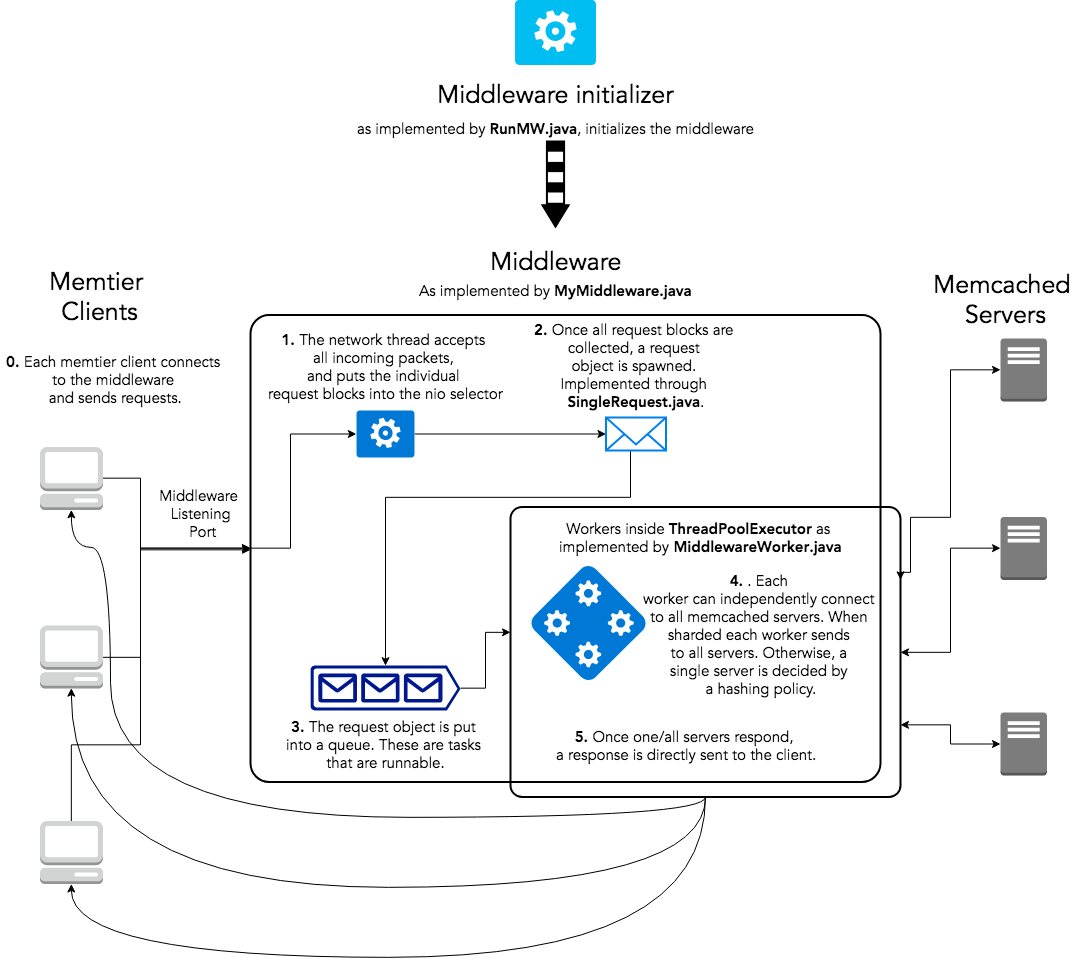
\includegraphics[width=\textwidth]{img/middleware_diagram.png}
\caption{Exp.2.1: A figure with two subfigures}
\label{fig:test}
\end{figure}


\begin{enumerate}
\item \textbf{scripts} \\
This folder includes all the logic to automatically compile the code, deploy the code, run the experiments (each individual one), and automatically download the logs.
This is true both for a local development environment (using docker VM's), and the external "production" environment (using Azure VM's). 
The local docker and external Azure systems are interchangable with a small change in command.

\item \textbf{data} \\
This folder includes all the raw data that is pulled from the experiment, all the python files which process upon this data, and all the processed data.

\item \textbf{figs} \\
This folder includes all the figures that are create using the processed data from point 2.
I use python to create figures from individual graphs

\item \textbf{src} \\
I will talk about the code structure of the src directory with more detail in this next section.
I take a top-down approach while explaining (i.e. starting with where requests originate, and where they go from there).
I will keep this consice, as the \textit{lifetime of a request} section covers some information on what happens in which file.

\begin{enumerate}
\item \textbf{RunMW.java} \\
This is the entry point / main class of the program.
This is the default implementation by the TA's.


\item \textbf{SingleRequest.java} \\
Is the class which encodes a single request from one of the clients.
This can include the SET or GET operation.
For logging purposes, this class also includes all possible times which may be of use to calculate the queueing theory (and latency and throughput) later on.

The request type is parsed by checking the very first character of the request string.
If the string starts with a "g", the request type is a GET (later on, it is decided on the fly if it is a MULTIGET by checking if the number of keys is greater than 1).
If the string starts with a "s", the request type is a SET.
If none of the above cases hold, an error happened (we exit gracefully, as this is unintended behavior).

\item \textbf{MyMiddleware.java} \\
This is the entrypoint of how the Middleware is called.
The datastructure we use to connect to the individual clients is the \textbf{nio.Selector}. 
The \textbf{nio.Selector} can hold multiple connections from different clients connecting. 
This datastructure can hold multiple keys for each connections, and fills up each key as long as the request is not done yet.
Once the request is complete, it will throw away that key and make space for a new connection.
Furthermore, it can parse packages that don't immediately fit into the bytebuffer.
The backlog size is bigger than 0 such that multiple requests can made to the same channel at the same time (and these requests are backlogged).


This class is responsible for fetching the individual requests (spawned as a \textit{SingleRequest} object)using non-blocking IO, putting it to a queue, and spawning \textit{MiddlewareWorker}'s within a \textbf{\textit{ThreadPool}} to act upon these requests.
We use the NIO selector to handle all connections.
The entire logic of this .java class runs in on the main thread of the class, which I may refer to as "Network Thread".
This allows for multiple clients to connect to the server in a non-blocking fashion.
Whenever a connection is compelte (i.e. the request is complete), this selector spawns a \textit{MiddlewareWorker} and a \textit{SingleRequest}.

The diagram above symbolizes how this works.

\item \textbf{MiddlewareWorker.java} \\
The \textit{MiddlewareWorker} takes a \textit{SingleRequest} and passes it to the server(s). 
The \textbf{MiddlewareWorker} implements \textbf{Runnable}, and is executed by the \textbf{ThreadPoolExecutor} by calling \textbf{submit}.
Depending on whether the request type is a SET or GET, we have different behavior:

\begin{itemize}
\item case SET: 
The \textit{SingleRequest} is sent to each individual server in a sequential manner.
After the sending to the server is done for all servers, it listens to the response of each individual server.
It listens until all servers have responded.
If any single item has responded with an error, this SET operation responds with the first error encountered to the client.
Otherwise it returns a \textbf{STORED} message. 

\item case GET: 
The string of the \textit{SingleRequest} is used to calculate a hash for the individual request.
This hash is then modulo-ed with the number of server that we can send the request to.
This is done to balance the read-workload amongst different memcached server instances.
The modulo operation decides which server to send it to.
This has \textbf{provenly uniformly at random distribution}  behavior (proof at: https:\/\/eprint.iacr.org\/2016\/985.pdf).
In short, this proof relies on the fact that hashing is pseudorandom, and that pseudorandomity means that for any input, all output values are uniformly at random distributed.
Pseudorandomity keeps it's properties when applied with the modulo operator. 
Because all operations preserve pseudorandomity, the final operation - and thus the server chosen - is also uniformly at random.

\item case MULTIGET (nonsharded):
The nonsharded multiget acts exactly like the GET case.
Again, the uniformly at random assumption is guaranteed because the hashing algorithm is pseudorandom (and as such provides keys uniformly at random).

\item case MULTIGET (sharded):
The sharded MULTIGET case acts as follows. The MULTIGET request is first split up into $n = max(keys, buckets)$ where $buckets$ is the number of servers in total, and $keys$ is the number of keys in total.
The split is sequentially, which means that the first thirds of the requests go to the first server, the second third go to the second server, etc.
Each individual split up request is then treated as an individual GET request.
When the memcached server responds, all the answers are concatenated in a sequential fashion and sent back to the client. 
Errors are handled and also reduced to the first occuring error if this is the case.
\end{itemize}


\item \textbf{LoggerUtils.java} \\
A helper class.
Includes all the logic that is needed to log the requests to hard disk.
All the request logic is accumulated to variables, and the mean is flushed to disk every few minutes.
For GET requests (and in the interest of experiment 5), GET requests are accumulated into a list, and flushed to disk every 5 seconds.
The logging happens in such a way that each individual \textit{MiddlewareWorker} has it's list of requests and all accumulater objects (inside the LoggerUtils.java) to be logged.
Because there is a separate Logger for each thread, there are no issues with multithreading as there is no concurrent data access. \\

Every single request keeps track of the following values, 
which is then flushed to the LoggerUtils.java (and thus to the file)
object when the request has been successfully.
All the information in SingleRequest is used to create the following log-informations.

\begin{enumerate}
\item timeRealOffset
\item differenceTimeCreatedAndEnqueued
\item differenceTimeEnqueuedAndDequeued
\item differenceTimeDequeuedAndSentToServer
\item differenceTimeSentToServerAndReceivedResponseFromServer
\item differenceTimeReceivedResponseFromServerAndSentToClient
\item timeRealDoneOffset
\end{enumerate}

\item \textbf{RequestType.java} \\
A helper struct definition, which defines the two possible input types (Multi-gets are decided on the fly at a different point as described in \textit{SingleRequest.java})

\end{enumerate}

\end{enumerate}

\subsection{Lifetime of a request}
In the following I will talk about how requests enter the middleware, how they are parsed, how they get distributed to servers, and how the middleware communicates these values back to the clients. 
This is a more detailed version of the above diagram.\\

\begin{enumerate}
\item \textbf{Request coming from client to middleware:}\\
When a request comes from a client to the middleware, I use an \textbf{nio.channels.Selector} to accept the request.
This datastructure has the following benefits.
First, it can distinguish between multiple clients.
Second, it can process these individual requests simultaneously in an asynchronous (non-blocking) manner.
Third, it fills up multiple channels (one for each connection, and thus, one for each client), which means that if the request does not fit into one network packet, it will just listen for the rest of the packet.
I detect if a single request fills up by filling a java \textbf{ByteBuffer} until it the request has come to an end (which we can recnognize by waiting for the \textbf{END} keyword.
We parse the type of request by looking at the very first character (interpreting the bytes) and cross-comparing if this is a \textit{set} or \textit{get}. 
To distinguish between \textit{multi-get} and \textit{gets}, we later on split the string resulting from parsing the bytebuffer by spaces.
If the number of elements after splitting is bigger than 2 (the "get" keyword, and the key), then I parse a multi-get.
Else, I parse a get.
\item \textbf{The incoming request spawns a SingleRequest object:}\\
The SingleRequest object is specified in the \textbf{SingleRequest.java} java file and is wrapped around a \textbf{MiddlewareWorker.java} object which implements a java \textbf{Runnable} on which I later on call \textbf{submit} using a \textbf{ThreadPoolExecutor}. 
This file keeps track of the statistics described in the LoggerUtils.java class for logging.
The SingleRequest takes over the \textbf{ByteBuffer} which was created while \textbf{nio.channels.Selector} was listening for a complete network packet.
This ByteBuffer will later on be passed to the individual server(s) (after some processing).
\item \textbf{Submitting a SingleRequest to a MiddlewareWorker using the java ThreadPoolExecutor}:\\
I use the SingleRequest that was generate before, and spawn a new MiddlewareWorker.
This MiddlewareWorker can then be submitted to the java \textbf{ThreadPoolExecutor} which contains the number of middleware-threads (as specified per experiment).
Each individual middlewareworker contains one instantiated \textbf{LoggerUtils} class per thread and thus is threadsafe.
\item \textbf{Sending the server response back to the client}: \\
Each middlewareworker, and thus each individual thread, has a connection to the client that the request came from, and a hashmap of sockets to connect to all the servers.
The response is sent back to the client using the description in the previous sub-section.
In any case, this goes through the individual middleware-worker thread, and does \textbf{not} go through the initial nio.channel.Selector again.
\end{enumerate}

\subsection{Some statistics, and observed bandwidths amongst different VMs}
I use the program \textit{iperf -c 'VM Address'} to arrive at these statistics.
I arrive at the theoretical maximum throughput by checking how many packages could possibly fit in the bandwidth, where the message size is 4KB (i.e. 4096 bytes), and the bandwidth is specified by the value before that.
I divide the bandwidth by the packet size to arrive at the theoretical maximum throughput per single VM.

\begin{center}
    \begin{tabular}{| l | l | l | l |}
    \hline
    VM From & VM To & Bandwidth & Theoretical Maximum Throughput per VM (ops/sec)\\ \hline
    Client & Middleware & 201 Mbits/sec &  6'250 \\ \hline
    Client & Server & 201 Mbits/sec & 6'250 \\ \hline
    Middleware & Client & 804 Mbits/sec & 25'000 \\ \hline
    Middleware & Server & 804 Mbits/sec & 25'000 \\ \hline
    Server & Client & 101 Mbits/sec &  3'125 \\ \hline
    Server & Middleware & 101 Mbits/sec & 3'125 \\
    \hline
    \end{tabular}
\end{center}

Intuitively, this means that if we have 3 clients and one server, the server must be a bottleneck, and that the clients share the $3'125 ops/s$ (approximately $1'000ops/s$ per client).
\textbf{I will use these numbers to derive some explanations later on}.\\

I am now talking about my statistical methods of how I analyse the experiments.
Each plotted value for each experiment in the subsequent report was generating using \textbf{three repetitions}, each including a \textbf{warm-up}, and a \textbf{cool-down} phase of 15 seconds (where the core-length of the experiment was 60 seconds).
For some experiments, I use a warm-up and cool-down time (respectively) of approximately 7 seconds, as my experiments became very lengthy at some point, and as this showed to give good results.
To arrive at a single rate amongst rates, I use the \textbf{arithmetic mean}, which is a common statistically significant measure.
As an \textbf{error mesaure}, I use the standard deviation, which is also a common statistically significant measure that is tightly coupled with the mean.
These are common statistical tools, and according to the \textbf{law of large numbers}, will approximate any distribution truthfully when the number of samples go against infinity, which is why I chose these two measures.
\textbf{Anytime I graph something, the mean of 3 (or more) trials will be used to mark then point. 
Errorbars are derived from the standard deviation}.
The mean $\mu$ and standard deviation $\sigma$ are calculated as follows:

\begin{equation}
\mu = \frac{\sum_i^n x_i} {n}
\end{equation}

\begin{equation}
\sigma = \sqrt{ \frac{\displaystyle\sum_{i=1}^{n}(x_i - \mu)^2} {n} }
\end{equation}

Please be aware, that I use the word \textit{client} to refer to the VM's that host the memtier instances, and the word \textit{server} to refer to the VM's that host the memcached instances.
Any virtual machine, I refer to as VM.

Whenever I speak about \textit{virtual client per thread}, I refer to the number of virtual clients per thread \textbf{per memtier instance}.
The reader should be able to infer that this number needs to be multiplied by the number of memtier-instance-threads to arrive at the total number of virtual clients.
I keep this concept constant, so comparison between experiments is sound.
In addition to that, I will use the words \textbf{latency} and \textbf{response time} interchangeably.
For the sake of easier typing, I will use approximate values (as far as reasonable), when it comes to discussions on throughput.

\newpage

\section{Baseline without Middleware (75 pts)}
These experiments don't use the middleware, and only consist of memtier client instances, and memcached server instances.
Each of these experiments have a warm-up time of 15 seconds, and a cool-down time of 15 seconds.
I Using high warm-up and cool-down times, I hope to get rid of manipulation of measurements by predominan non-core phases.

\subsection{One Server}

I use the following setup:

\begin{center}
	\scriptsize{
		\begin{tabular}{|l|c|}
			\hline Number of servers                & 1                        \\ 
			\hline Number of client machines        & 3                        \\ 
			\hline Instances of memtier per machine & 1                        \\ 
			\hline Threads per memtier instance     & 2                        \\
			\hline Virtual clients per thread       & [1..32]                  \\ 
			\hline Workload                         & Write-only and Read-only \\
			\hline Repetitions                      & 3 or more                \\ 
			\hline 
		\end{tabular}
	} 
\end{center}

I will test out the response time and latency for a different number of virtual clients per thread on the client-side (per memtier instance), namely [1, 2, 4, 8, 16, 32].
I will talk about read-only operations, and write-only operations.
As there is no difference in pre-populating the servers in the case of writes, for both experiments I pre-populate the server the same way as using the following command, which sequentially generates and stores each key in the server.
\textbf{Wheneverin future experiment setups  I refer to prepopulating the server, I will refer to this command}:

\begin{spverbatim}
      memtier_benchmark -s {SERVER_IP} -p {PORT}
      --protocol=memcache_text --clients={VIRTUAL_CLIENTS_PER_THREAD} --threads={THREADS}
      --requests=15000 --ratio=1:0 --data-size=4096
     --expiry-range=9999-10000 --key-maximum=10000 --key-pattern=S:S
\end{spverbatim}
.\\
The clients and servers don't use multi-gets, and there is no middleware involved.
I run 3 repetitions of each configuration and plot the mean and standard deviation of the trials for each possible configuration. \\

\begin{figure}[H]
\centering
\begin{subfigure}{.5\textwidth}
    \centering
    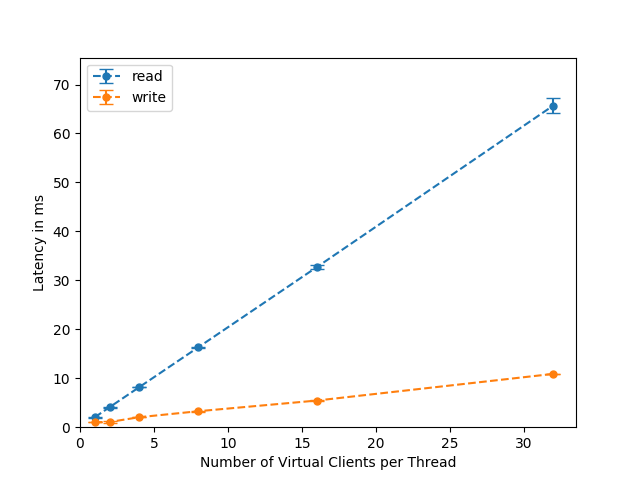
\includegraphics[width=\textwidth]{img/exp2_1/exp2_1__latency_client_read_write.png}
    \caption{Latency}
    \label{fig:mesh1}
\end{subfigure}%
\begin{subfigure}{.5\textwidth}
      \centering
    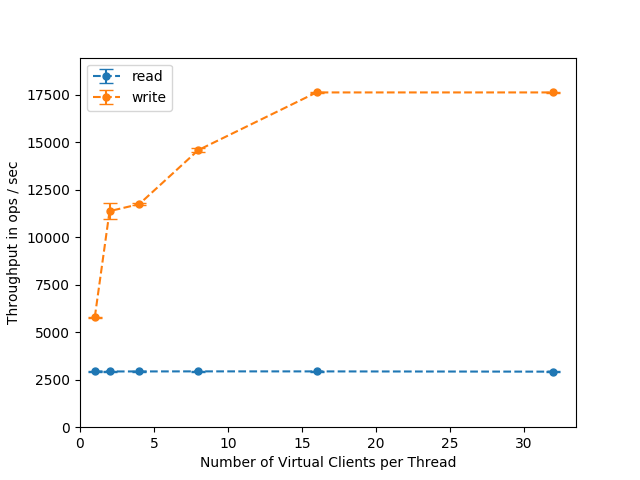
\includegraphics[width=\textwidth]{img/exp2_1/exp2_1__throughput_client_read_write.png}
    \caption{Throughput}
    \label{fig:mesh1}
\end{subfigure}
\caption{Exp.2.1: Latency and Throughput per number number of virtual clients per memtier-thread. Comparison of read-only and write-only values.}
\label{fig:test}
\end{figure}


For the \textbf{read-only experiments}, the system becomes saturated even with 1 virtual client per thread (per memtier instance), and does not oversaturate as the system is stable.
This is because the throughput reached approximately almost $3000ops/s$, which conforms to the observation of the maximum theoretical throughput per \textbf{server} in section 1 (minus some network overhead).

This stability is indicated by the error (which is very small, and thus for some points intersects with the measured points).
The error metric (standard deviation) is explained in section 1.\\

For the \textbf{write-only experiments} the system (in this case the server), is undersaturated until 16 virtual clients per memtier-threads, after which it reaches a stable saturated phase, and never reaches over-saturation (due to stability of the system).
This stability of the system is indicated by the small error bars, (which are hardly readable for this reason)
This is because the throughput reached approximately almost $18000ops/s$ at 16 virtual clients per memtier-threads, and is increasing to this number before that, which conforms to the observation of the maximum throughput per \textbf{server} in section 1.\\

As a sanity check, the interactive law holds, as the throughput flattens out after a square-root-like growth, while the response time still increases linearly.

For \textbf{read-only operations}, the bottleneck is the upload bandwidth of the server,
as 3 clients are trying to download a load of 100Mbit/s, and thus must each share appr. 33Mbit/s.
This corresponds to the total upload bandwidth of $3000ops/sec$ (which was empirically proven in section 1 through an additional experiment), is thus divided amongst  three servers.
This also proves to be a valuable sanity check.
As the number of threads increases, more requests are able to be generated.
Because the network bandwidth stays constant, but we introduce more virtual clients, the round-trip time of individual requests increases.
This implies a linear increase in latency, as can be seen from the graph.
This linear increase in the response time provides a third sanity check.

For \textbf{write-only operations}, the bottleneck is the upload bandwidth of the thee clients,
as 3 clients are trying to upload a load of 200Mbit/s each.
The server only responds with message suchs \textit{STORED}, which take up almost no bandwidth compared to the actual message itself.
Thus, the total bandwidth is the additive bandwidth of each individual client, which means approximately $ 3 \times 200 Mbit/s = 600 Mbit/s $, which corresponds to approximately $18000 ops/sec $ (same calculation as in section 1.2). 
This also proves to be a valuable sanity check.
I know that storing the individual requests is not the bottleneck, as a local docker experiment proves that higher throughputs can be achieved locally.
The clients are not able to generate enough load with 1, 2 or 4 virtual clients per thread, and only generate a maximum load with 16 virtual clients per threads, where the system finally saturates the upload bandwidth of the client VMs.
This can also be seen from the graph, which plateaus around 16 virtual clients per thread.
As a sanity check, the latency graph shows how the latency barely increases for up to 4 virtual clients per thread.
Only after the 4th virtual client per thread, does the response time increase linearly, which underlines the saturation phase.

\subsection{Two Servers}

I use the following setup:

\begin{center}
	\scriptsize{
		\begin{tabular}{|l|c|}
			\hline Number of servers                & 2                        \\ 
			\hline Number of client machines        & 1                        \\ 
			\hline Instances of memtier per machine & 2                        \\ 
			\hline Threads per memtier instance     & 1                        \\
			\hline Virtual clients per thread       & [1..32]                  \\ 
			\hline Workload                         & Write-only and Read-only \\
			\hline Repetitions                      & 3 or more (at least 1 minute each)                \\ 
			\hline 
		\end{tabular}
	} 
\end{center}

I will test out the response time and latency for a different number of virtual clients per thread on the client-side (per memtier instance), namely [1, 2, 4, 8, 16, 32].
As there is no difference in pre-populating the servers in the case of writes, for both experiments I pre-populate the server the same way as in experiment 2.1 (Baseline without middleware and 3 clients).
The clients and servers don't use multi-gets, and there is no middleware involved.
I run 3 repetitions of each configuration, each having a length of 90 seconds (such that the warm-up and cool-down times of 15 seconds respectively even out). \\

\begin{figure}[H]
\centering
\begin{subfigure}{.5\textwidth}
    \centering
    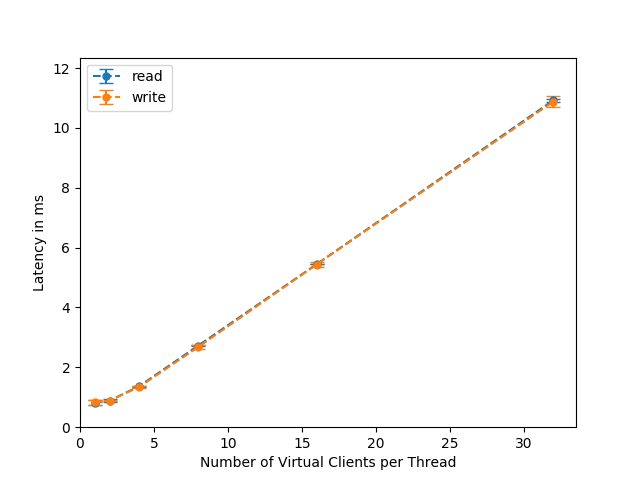
\includegraphics[width=\textwidth]{img/exp2_2/exp2_2__latency_client_read_write.png}
    \caption{Latency}
    \label{fig:mesh1}
\end{subfigure}%
\begin{subfigure}{.5\textwidth}
      \centering
    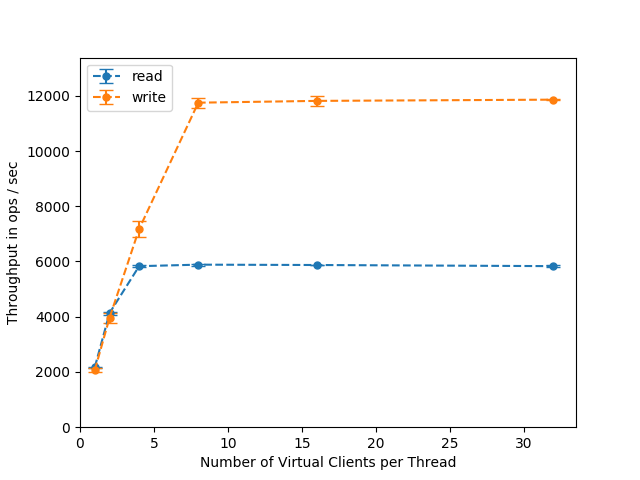
\includegraphics[width=\textwidth]{img/exp2_2/exp2_2__throughput_client_read_write.png}
    \caption{Throughput}
    \label{fig:mesh1}
\end{subfigure}
\caption{Exp.2.2 Latency and Throughput per number of virtual clients per memtier-thread. Comparison of read-only and write-only values.}
\label{fig:test}
\end{figure}

For  \textbf{throughput for the read-only experiments} both server virtual machine, are using their maximum capacity to upload all the values that are uploaded by the server virtual machines.
The combined throughput of the two servers is $2 \times 100Mbit/s$ which corresponds to a compound $200Mbit/s$.
This conform to the maximum theoretical throughput of $6000ops/sec$ when using the same calculation as in section 1.2.
The graph underlines these observed values.

For \textbf{throughput for write-only experiments}m the server can respond fast enough to all requests by the clients, because the response message (which is usually "STORED") consumes almost none of the bandwidth. 
Both memtier instances are using their maximum capacity to upload all the values to from the \textit{client} machine, to the server virtual machines.
The system is undersaturated initially as the clients cannot create enough load, and then becomes saturated after an increase of virtual client threads.
This can be seen from the plot which indicates that there is minimal to no oversaturation (there is a slight decrease in throughput, but is below some error measures).
The inflection point can be seen on the graphs at 4 virutal clients per memtier-thread.
The repsonse times start to become more steeper after this point, and the throughput flats out.
This conform to the $6000ops/sec$ when using the same calculation as in section 1.2.\\
For \textbf{read-only operations}, the bottleneck is the upload bandwidth of the server virtual machines, as each server is uploading 100Mbit/s each, which compounds to 200Mbit/s together.
The total upload bandwidth of 6000ops/sec (which was empirically proven in section 1 through an additional experiment), is thus divided amongst amongst two memtier servers and thus two memtier instances on the same machine (as can be seen in the client logs).
This also proves to be a valuable sanity check.
For up to 4 virtual clients per threads, the response time stays constant, simply due to the fact that the bandwidth is not saturated, and the requests don't have to wait on each other to be processed (but can be processed in parallel).
This implies an almost constant latency for up to 4 virtual clients per thread, and then an increase in latency, as can be seen from the graph. \\
For \textbf{write-only operations}, the bottleneck is the upload bandwidth of the client virtual machines, as the single client is uploading 200Mbit/s each, which compounds to 200Mbit/s together.
Once the client spawns 4 virtual clients per thread, the client VM upload bandwidth starts to saturate as the client upload bandwidth of 200Mbit/s is reached, as each memtier instance in the client is actually able to generate approximately $3'000 ops/sec$, which compounds to $6'000 ops/sec$ when ran on two memtier instances.
Because the network bandwidth stays constant, the round-trip time of individual requests increases, except for up to 4 virtual clients per thread.
For up to 4 virtual clients per threads, the response time grows slowly, simply due to the fact that the bandwidth is not saturated, and the requests don't have to wait on each other to be processed (but can be processed in parallel).\\

Both read-only and write-only operations are stable, as can be seen from the very small (and this barely readable) error metric.
Furthermore, the interactive law holds for both experiments, as the throughput flattens out after 4 virtual clients, while the latency starts increasing.
This servers as a sanity check. \\


\subsection{Summary}

The following table summarizes the quantiative results. I then compare the read-only and write-only workloads.
This is a summary. 
Because this report is meant to be concise, for any explanations, please see the above sections.

\begin{center}
	{Maximum throughput of different VMs.}
	\begin{tabular}{|l|p{2cm}|p{2cm}|p{4cm}|}
		\hline                        & Read-only workload & Write-only workload & Configuration gives max. throughput \\ 
		\hline One memcached server   & 2940 & 17633 & VC=16  \\ 
		\hline One load generating VM & 5939 & 6054 & VC=8 \\ 
		\hline 
	\end{tabular}
\end{center}

I first compare read-only and write-only operations.
I start with \textbf{read-only operations} first.
For \textbf{one memcached server and three clients}, the bottleneck is the server, which is bottlenecked to serve at most $3'000 ops/sec $.
In contrast, using \textbf{one load generating VM}, the bottleneck is the upload bandwidth of upload bandwidth of the server (2 times the upload bandwidth of a server) $6'000 ops/sec$. 
In both cases, a bottleneck occurs exactly if the messages take over the entire network/upload bandwidth, and never happens when only messages such as "GET" or "STORED" are sent back.
The bottleneck as such is the same for both configurations, being the server which must send enough data back to the client.
I continue with \textbf{write-only operations}.
For \textbf{one memcached server and three clients}, the bottleneck is the client, as the server has a response which virtually fills none of the bandwidth.
For \textbf{one load generating VM}, the bottleneck is the upload bandwidth of the client, as the client cannot generate more than $6'000 ops/sec$ of bandwidth-filled requests.
The bottleneck as such is the same for both configurations, being the client which mus send enough data to the server (to be stored). 
All these values conform to the measurement done in section 1.\\

I proceed with comparing the two server configurations.
For \textbf{one memcached server}, any read-operation is bottlenecked by the number of servers, because we only have one server, this value can maximally achieve $3'000 ops/sec$.
For any write-only operations, the bottleneck is the number of clients. 
Because we have 3 clients, this value can maximally achieve $18'000 ops/sec$.
The compound upload bandwidth of the client machines is at approximately $3 \times 200 Mbit/s$, whereas the compound upload bandwidth of the server machines is approximately $100 Mbit/s$.
This means that the clients can send almost any load of operations they want.
In contrast, write-operations don't suffer this penalty, as the server has almost no bandwidth to give away, as in this case the server only responds with "STORED", and never with a datapacket which is of size $4KB$ (which would fill the bandwidth). 

For \textbf{one load-generating}, any read-operations are bottlenecked by the number of servers. Because there is always 2 servers, the maximal throughput is $t6'000 ops / sec$.
Any write-operation is again bottlenecked by the number of clients.
Because we have one client, this value is capped by the $6'0000 ops / sec$.

For one memecached server, the "balance" is heavily destroyed, whereas one can see that one client and two servers both can handle the same volume in throughput.
As such, the configuration with only one memcached server, and the configuration with one load generating VM are in polar contrast to each other, showing that the servers have relatively few bandwidth compared to the client machines, but that the server is fast enough for as long as the operation is only a sending a simple "STORE" (i.e. bandwidth is not fully used up).

Any numbers that deviate from the theoretical maximum arise due to network overhead, and are statistically insignificant in this analysis.

\section{Baseline with Middleware (90 pts)}

\subsection{One Middleware}

In this set of experiments, I use three client memtier virtual machines, and 1 memcached server.
These virtual machine instances are connected with exactly one middleware virtual machine in the middle.
The three clients connect to the middleware. 
The middleware connects to the server.
For this section, I repeat each experiment for 3 times and plot the standard deviation amongst those trials.
I also allow for a 15 second warm-up and 15 second cool-down time, and disregard these measurements when retrieving the logs about the request times from the middleware.
I measuring the throughput and response time for different values of number of virtual clients.

\begin{center}
	\scriptsize{
		\begin{tabular}{|l|c|}
			\hline Number of servers                & 1                        \\ 
			\hline Number of client machines        & 3                        \\ 
			\hline Instances of memtier per machine & 1                        \\ 
			\hline Threads per memtier instance     & 2                        \\
			\hline Virtual clients per thread       & [1..32]                  \\ 
			\hline Workload                         & Write-only and Read-only \\
			\hline Number of middlewares            & 1                        \\
			\hline Worker threads per middleware    & [8..64]                  \\
			\hline Repetitions                      & 3 or more (at least 1 minute each)                \\ 
			\hline 
		\end{tabular}
	} 
\end{center}

The setup is exactly the same as in experiment "Baseline without Middleware and 1 server", with the difference that we inject one middleware between the 3 clients and the server.
In addition to the virtual clients per thread, I also investigate how the joint modification of the middleware-threads influences the latency and throughput.
I test out the throughput and latency for any permutation of
virtualthreads=[1, 2, 4, 8, 16, 32] and threads in the middleware=[8, 16, 32, 64].

I first separately investigate \textbf{read-only operations} and \textbf{write-only} operations, and arrive at a comparison between these four systems in the summar in section 3.3.

Any graph involving the middleware stripped out the operations that happened during the warm-up and cool-down times.
\textbf{For the sake of conciseness, I had to collapse the multiple plots into one single plot, even though the measurements overlap to a high degree.}

\subsubsection{Read-only}

I first plot the latency and response as measured on the middleware.

\begin{figure}[H]
\centering
\begin{subfigure}{.5\textwidth}
    \centering
    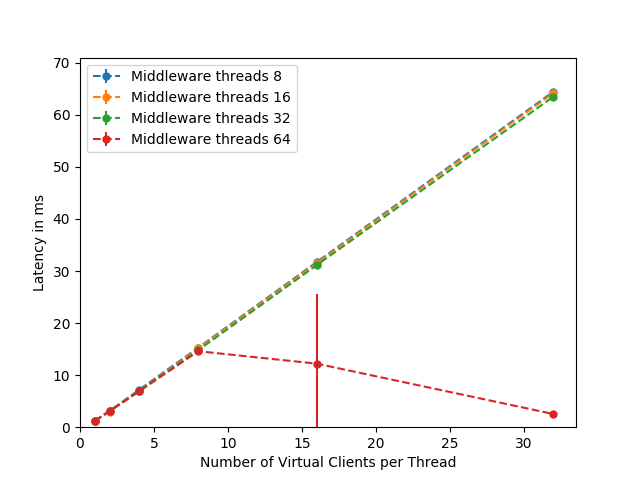
\includegraphics[width=\textwidth]{img/exp3_1/exp3_1__latency_middleware_write_0.png}
    \caption{Latency}
    \label{fig:mesh1}
\end{subfigure}%
\begin{subfigure}{.5\textwidth}
      \centering
    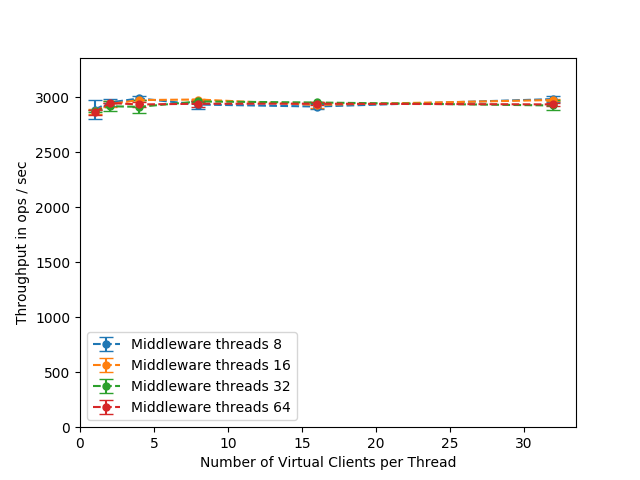
\includegraphics[width=\textwidth]{img/exp3_1/exp3_1__throughput_middleware_write_0.png}
    \caption{Throughput}
    \label{fig:mesh1}
\end{subfigure}
\caption{Exp3.1: Latency and throughputs for \textbf{read-only} as measures by the \textbf{middleware} (one middleware)}
\label{fig:test}
\end{figure}

For read-only operations, the bottleneck is the upload bandwidth of the server,
as 3 clients are trying to download a load of 200Mbit/s, and thus must each share appr. 66Mbit/s per machine.
This translates to appr. $1000 ops/sec$ per machine, or in other words $3000ops/s$ total throughput.
The throughput graph supports this claim.
As a sanity check, this conforms to the observation of the maximum throughput per server in section 1.
The middleware is no bottleneck even with only 8 middleware threads, because the results do not deviate from the results in section 2.1 (where the only difference is that we are addding a mdidleware between the clients and the server).
Another obvervation supporintg this claim stems from the fact that increasing the number of middleware threads does no increase performance.
The graphs support this claim.
The middleware virtual machine does not slow this down, as all GET requests are very short simple requests that all fit into the buffer.
Also, the IO that serves as input to the middleware is non-blocking, which means that it can accept many such small requests simultaneously.
This can be seen as increasing the number of middleware threads does not affect performance, as the server-side is bottlenecked.
Each individual request is sent back to the client. 
But because all threads have designed channels to the respective clients, and because the bandwidth of the server is so low compared to the bandwidth of the middleware virtual machine, this causes no slowdown.

The system is very stable, as can be noticed by the error which is again very small, and thus barely readable around the measured points.
As another sanity check, I present the throughput and latency plots from the \textbf{client machines}, which all conform to the throughputs and latencies as caluclated in the middleware.
To keep it concise, and because these graphs heavily look like the middleware graphs, I include these in the appendix. 

\begin{figure}[H]
\centering
\begin{subfigure}{.5\textwidth}
    \centering
    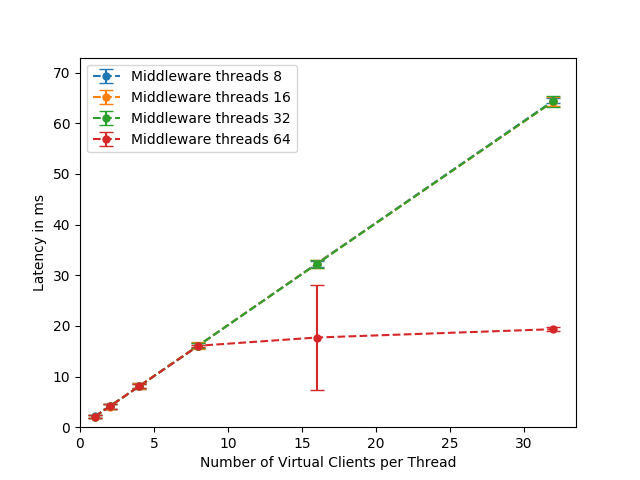
\includegraphics[width=\textwidth]{img/exp3_1/exp3_1__latency_client_write_0.png}
    \caption{Latency}
    \label{fig:mesh1}
\end{subfigure}%
\begin{subfigure}{.5\textwidth}
      \centering
    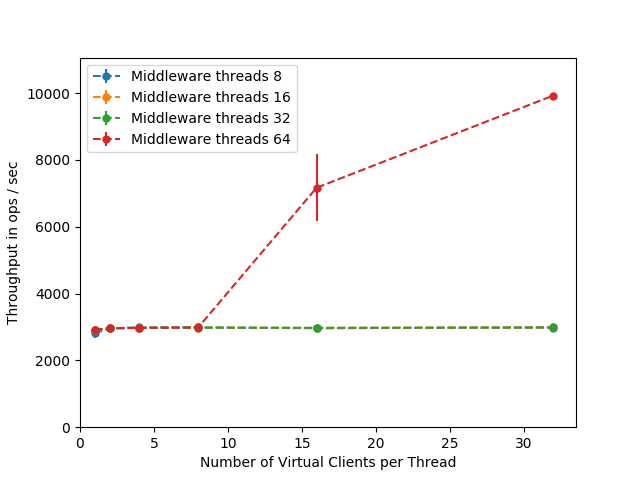
\includegraphics[width=\textwidth]{img/exp3_1/exp3_1__throughput_client_write_0.png}
    \caption{Throughput}
    \label{fig:mesh1}
\end{subfigure}
\caption{Exp3.1: Latency and throughputs for \textbf{read-only} as measured by the \textbf{clients} (combined throughput)}
\label{fig:test}
\end{figure}


As the number of threads increases, more requests are able to be generated.
Because the network bandwidth stays constant, the round-trip time of individual requests increases.
The clients are able to generate enough load with even 1 virtual client per thread, such that with 1 virtual thread the network bandwidth is saturated at a very early stage with 1 virtual client per memtier thread.
This implies an increase in latency.
The linear increase in the latency graph supports this claim.
As a last sanity check, one can confirm that the interative law holds.
The throughput flattens out, as the response time increases.
This claim is supported by the graphs.


\subsubsection{Write-only}

I first plot the latency and response as measured on the middleware.

\begin{figure}[H]
\centering
\begin{subfigure}{.5\textwidth}
    \centering
    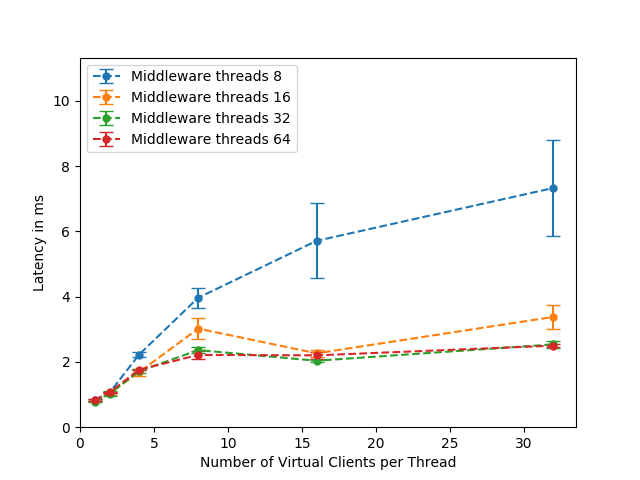
\includegraphics[width=\textwidth]{img/exp3_1/exp3_1__latency_middleware_write_1.png}
    \caption{Latency}
    \label{fig:mesh1}
\end{subfigure}%
\begin{subfigure}{.5\textwidth}
      \centering
    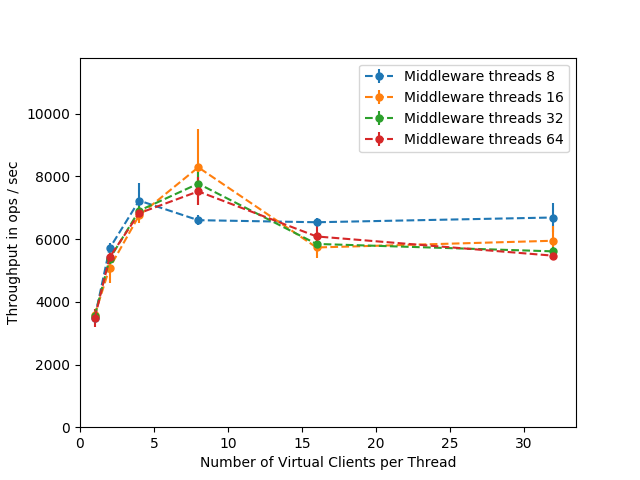
\includegraphics[width=\textwidth]{img/exp3_1/exp3_1__throughput_middleware_write_1.png}
    \caption{Throughput}
    \label{fig:mesh1}
\end{subfigure}
\caption{Exp3.1: Latency and throughputs for \textbf{write-only} as measures by the \textbf{middleware} (one middleware)}
\label{fig:test}
\end{figure}

The bottleneck is the middleware, as the performance increases until 8 virtual clients per threads, and then sharply drops due to the oversaturation of the incoming requests.
This claim is supported by the fact, that 8 middleware-threads has the lowest performance, and increasing the number of middlewarethreads increases the throughput.
Especially the response graph supports this claim.
Another explanation for this is that the middleware reaches a throughput of approximately $8'000 ops/sec$, which is much lower than the theoretical maximum of $18'000 ops/sec$, as measured in experiment 2.1.
The only factor we changed is adding the middleware, so the middleware must be the delimiting factor.
Another reason why this is the case is that the network bandwidth is not a delimiting factor for this, as we know from experiment 2.1 that the client maximum throughput for this specific configuration would usually almost be $18'000 ops/sec$, and also because I know that the server only responds with "STORED", which take up almost no bandwidth at all.
This claim is supported by the fact that the middleware virtual machines do allow an upload bandwidth of $25'000 ops / sec$, which should easily be able to hand the theoretical maximum total upload throughput of the client machines of $18'000 ops/sec$.
In the next experiment (3.2), I will continue to show that this claim is true.

The middleware is under-saturated until 4 virtual clients per memtier thread, and is saturated after this point.
There is no real over-saturation, as the middleware does not decrease in performance, but keeps stabily this throughput rate.
The throughput graph, which increases in throughput until 4 virtual clients per thread, and then (only slowly) increases and almost stays constant supports this claim.

The experiments are still stable, but do have higher variance than all previous experiments, which stems from the fact that a single machine must now be responsible for a very high throughput (instead of distributing this load across multiple virtual machines).
This can be seen from the higher errobars (compared to previous experiments).

To apply some sanity checks, I observers the latency and throughput graphs as measured by the client. 
The client takes into account additional network roundtrip time, which makes the response graph as measure by the client slightly different.
The throughput graph confirms the middleware's throughput rates, however.
This can be seen in the following graphs.

\begin{figure}[H]
\centering
\begin{subfigure}{.5\textwidth}
    \centering
    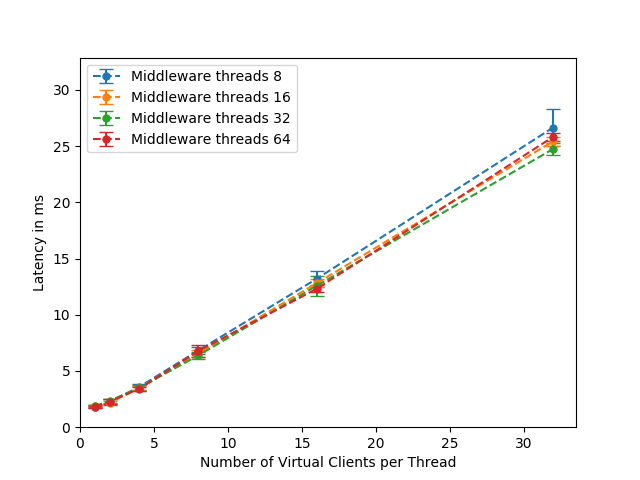
\includegraphics[width=\textwidth]{img/exp3_1/exp3_1__latency_client_write_1.png}
    \caption{Latency}
    \label{fig:mesh1}
\end{subfigure}%
\begin{subfigure}{.5\textwidth}
      \centering
    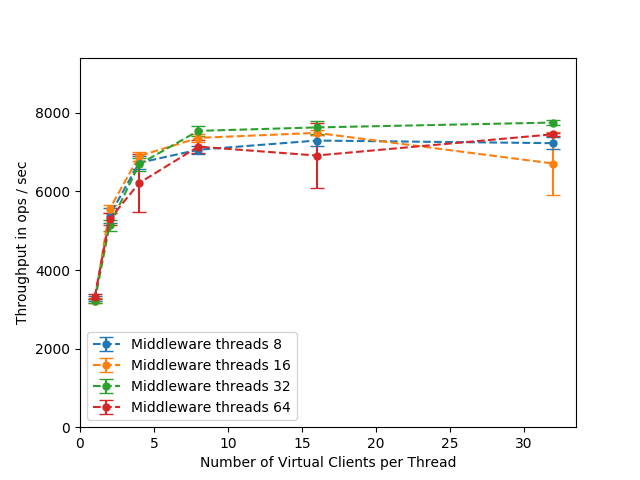
\includegraphics[width=\textwidth]{img/exp3_1/exp3_1__throughput_client_write_1.png}
    \caption{Throughput}
    \label{fig:mesh1}
\end{subfigure}
\caption{Exp3.1: Latency and throughputs for \textbf{write-only} as measures by the \textbf{clients} (one middleware)}
\label{fig:test}
\end{figure}


As a final sanity check, the throughput increases and then stays constant, while the throughput constantly increases.
This indicates that the interactive law applies.
This is also supported by the graphs.

\subsubsection{Additional Explanation}

I analyse the average size of the queue inside the middleware, and also investigate response times as a function of \textit{middleware threads} and \textit{virtual clients per memtier thread}.
The graphs of the response times can be found in the appendix, for conciseness.

\begin{figure}[H]
\centering
\begin{subfigure}{.5\textwidth}
    \centering
    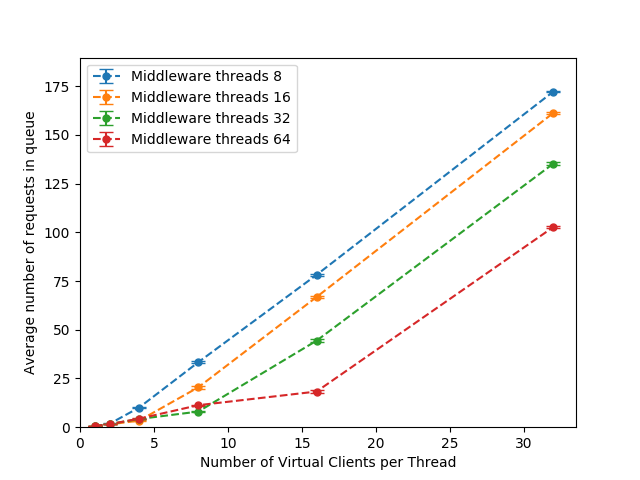
\includegraphics[width=\textwidth]{img/exp3_1/exp3_1__queuesize_middleware_write_0.png}
    \caption{Read-only}
    \label{fig:mesh1}
\end{subfigure}%
\begin{subfigure}{.5\textwidth}
      \centering
    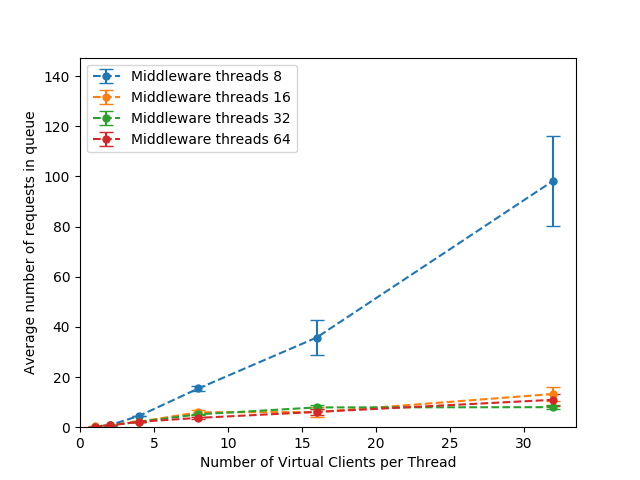
\includegraphics[width=\textwidth]{img/exp3_1/exp3_1__queuesize_middleware_write_1.png}
    \caption{Write-only}
    \label{fig:mesh1}
\end{subfigure}
\caption{Exp3.1: Average Queuesize in middleware \textbf{per} number of middleware threads and \textbf{per} virtual cliens per memtier thread}
\label{fig:test}
\end{figure}

For write-operations, the queue contains the message that is to be written.
This means that if the requests cannot be handled fast enough, the queuesize will increase.
If the requests can be handled fast enough though, the queue-size will stay at a low constant value.
For read-only requests, there is almost no bottleneck, which means that the queuesize amongst all middleware-workers is similar.
The queuesize increases with an increasing number of virtual clients per threads, but because the all the queuesizes (across a different number of middleware-threads) increase together, this shows that the middlewareworker is no bottleneck.
The read-only average queuesize graph supports this claim.

For write-only requests, however, 8 middleware threads are not as performant as more number of middleware threads.
This can easily be seen from the queuesize graph for write-only operations.
This graph shows that the queuesize steeply increases for 8 middleware-threads, but stays similar across higher middleware thread-counts.

As the number of virtual clients per threads increases, the latency is shifted more and more  from "waiting for the server", to "waiting in the queue", as the wait-time and service-time graphs in the appendix show.
This implies that the middleware congests the requests and collects the requests in the queue as it is not able to process all requests fast enough.

\subsection{Two Middlewares}

In this set of experiments, I use three client memtier virtual machines, and 1 memcached server.
These virtual machine instances are connected with exactly two middleware virtual machines in the middle.
The three clients connect to the middlewares (two memtier-instances per client machine). 
The middlewares both connect to the server.
For this section, I repeat each experiment for 3 times and plot the standard deviation amongst those trials.
I also allow for a 15 second warm-up and 15 second cool-down time, and disregard these measurements when retrieving the logs about the request times from the middleware.
I measuring the throughput and response time for different values of number of virtual clients.

\begin{center}
	\scriptsize{
		\begin{tabular}{|l|c|}
			\hline Number of servers                & 1                        \\ 
			\hline Number of client machines        & 3                        \\ 
			\hline Instances of memtier per machine & 2                        \\ 
			\hline Threads per memtier instance     & 1                        \\
			\hline Virtual clients per thread       & [1..32]                  \\ 
			\hline Workload                         & Write-only and Read-only \\
			\hline Number of middlewares            & 2                        \\
			\hline Worker threads per middleware    & [8..64]                  \\
			\hline Repetitions                      & 3 or more (at least 1 minute each)                \\ 
			\hline 
		\end{tabular}
	} 
\end{center}

The setup is exactly the same as in experiment "Baseline without Middleware and 1 server", with the difference that we inject two middlewares between the clients, and the server.
Another difference is that we allow each individual client to run two memtier instances (each with one thread) to be able to connect to two instances each.

In addition measuring the throughput and response time for different values of number of virtual clients, we also allow to modify the number of middleware threads as another measureable variable.
This means that I test out the throughput and latency for any permutation of
virtualthreads=[1, 2, 4, 8, 16, 32] and threads in the middleware=[8, 16, 32, 64].\\

I first talk separately about read-only operations, write-only operations, and then compare them in another section subsubsection "Additional Explanation".

\subsubsection{Read-only}
I first start with read-only operations.

\begin{figure}[H]
\centering
\begin{subfigure}{.5\textwidth}
    \centering
    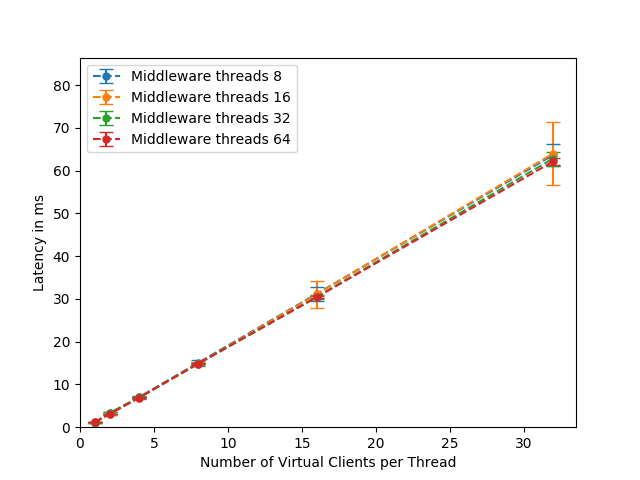
\includegraphics[width=\textwidth]{img/exp3_2/exp3_2__latency_middleware_write_0.png}
    \caption{Latency}
    \label{fig:mesh1}
\end{subfigure}%
\begin{subfigure}{.5\textwidth}
      \centering
    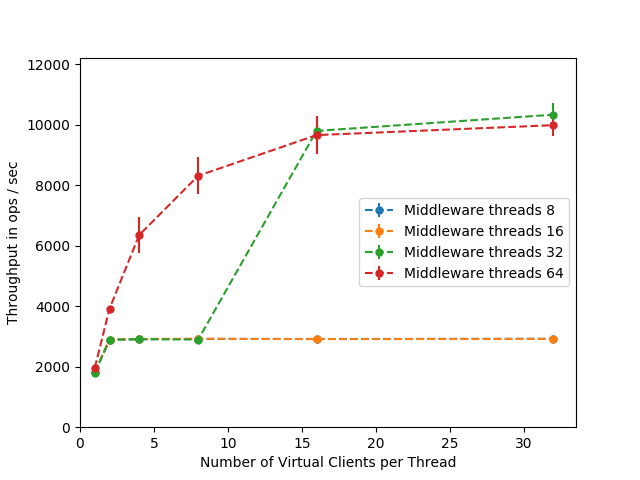
\includegraphics[width=\textwidth]{img/exp3_2/exp3_2__throughput_middleware_write_0.png}
    \caption{Throughput}
    \label{fig:mesh1}
\end{subfigure}
\caption{Exp3.2: Latency and throughputs for \textbf{write-only} as measures by the \textbf{middlewares} (two middlewares)}
\label{fig:test}
\end{figure}

For read-only workloads, the bottleneck is the server, with the very same explanation as in  section 3.1.
Please refer to section 3.1, as I will not repeat this explanation here for conciseness.
Because we introduce no additional server, this bottleneck does not change, and the maximum number of ops / sec does not increase.
This claim is supported by the throughput graph, which shows that the system is already saturated with 2 virtual clients per thread.
Introducing the second middleware does not improve this performance, as the number of servers does not change.

As such, the system saturates already with 2 virtual clients per memtier thread - the same as in experiment 2.1 read-only and experiment 3.1 read-only.
There is no oversaturation, and the system is stable, as can be seen from the slight error bars in both the response graph, and the throughput graph.

As a sanity check, one the interactive law applies, as the latency grows although the throughput stays the same.
In addition to that, the throughput and response time graphs as measure by the client support the throughputs as observed in the middleware.

\begin{figure}[H]
\centering
\begin{subfigure}{.5\textwidth}
    \centering
    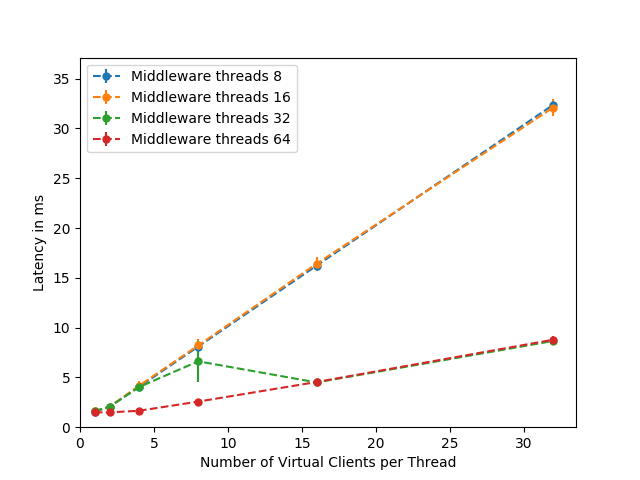
\includegraphics[width=\textwidth]{img/exp3_2/exp3_2__latency_client_write_0.png}
    \caption{Latency}
    \label{fig:mesh1}
\end{subfigure}%
\begin{subfigure}{.5\textwidth}
      \centering
    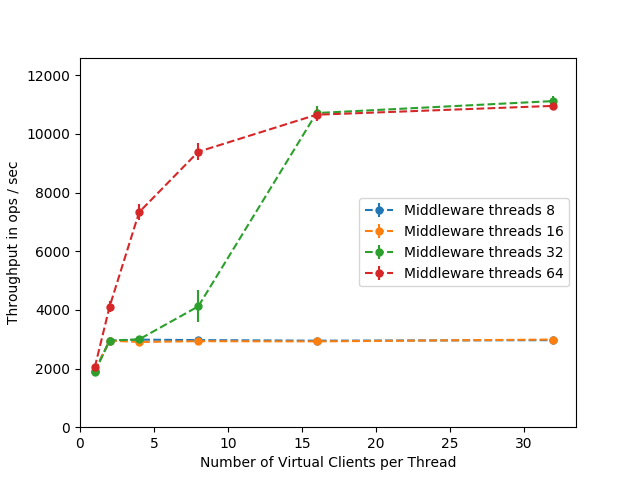
\includegraphics[width=\textwidth]{img/exp3_2/exp3_2__throughput_client_write_0.png}
    \caption{Throughput}
    \label{fig:mesh1}
\end{subfigure}
\caption{Exp3.2: Latency and throughputs for \textbf{write-only} as measures by the \textbf{clients} (two middleware)}
\label{fig:test}
\end{figure}

\subsubsection{Write-only}

I proceed with write-only operations.

\begin{figure}[H]
\centering
\begin{subfigure}{.5\textwidth}
    \centering
    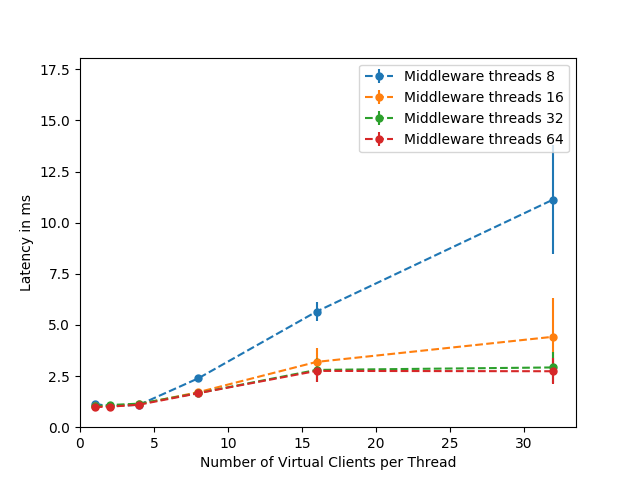
\includegraphics[width=\textwidth]{img/exp3_2/exp3_2__latency_middleware_write_1.png}
    \caption{Latency write only}
    \label{fig:mesh1}
\end{subfigure}%
\begin{subfigure}{.5\textwidth}
      \centering
    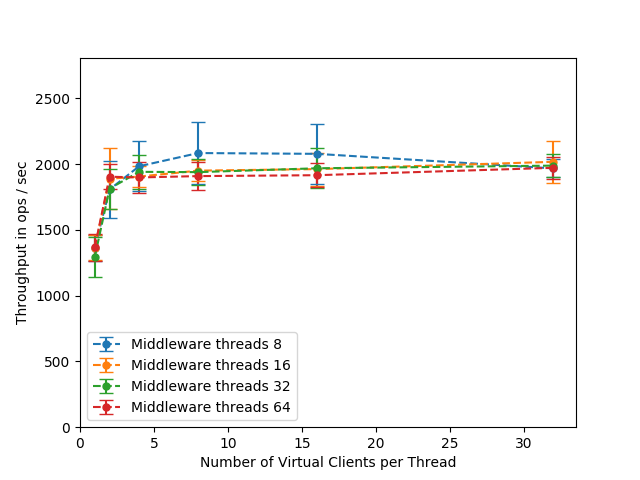
\includegraphics[width=\textwidth]{img/exp3_2/exp3_2__throughput_middleware_write_1.png}
    \caption{Throughput write only}
    \label{fig:mesh1}
\end{subfigure}
\caption{Exp3.2: Latency and throughputs as measures by the middlewares}
\label{fig:test}
\end{figure}

For read-only workloads, the bottleneck is the middleware instance, as was explained in section 3.1 write-only.
Please refer to section 3.1 for an explanation on this.
Because the middleware is the bottleneck, one can clearly see that for write-only operations, adding the second middleware almost doubles the throughput of the system.
This is because the total load of the system is now distributed amongst two middlewares instead of only a single one.
This means that each in total, we have double the amount of middleware-threads that can handle the requests.
This claim is supported by comparing the write-only graphs in this section with the write-only graphs in section 3.1.
One can validate, that doubling the number of threads in the middleware (which can be achieved by also by just spawning a second middleware which takes over part of that load), the throughput increases significantly. \\

The bottleneck is the total number of middlewarethreads in the system.
For 8 and 16 middleware threads per middleware instance, the system is under-saturated up to 8, respectively 16 virtual clients per thread. 
For a higher number of middleware-threads per middleware instance, increasing the number of virtual clients per thread almost allows to reach the system the maximum throughput as is given by the compound throughput of the client machines.
This claim is supported by the graph which shows an evening out of the throughput rate after 16 virtual clients per thread for 8 and 16 middleware threads per middleware instance, and an square-root-like increase in the throughput of the system which have 32 and respectively 64 middleware threads per middleware. \\

As a sanity check, one the interactive law applies, as the latency grows although the throughput stays the same, and this with an ever-increasing rate.
In addition to that, the throughput and response time graphs as measure by the client support the throughputs as observed in the middleware as the following graphs show.

\begin{figure}[H]
\centering
\begin{subfigure}{.5\textwidth}
    \centering
    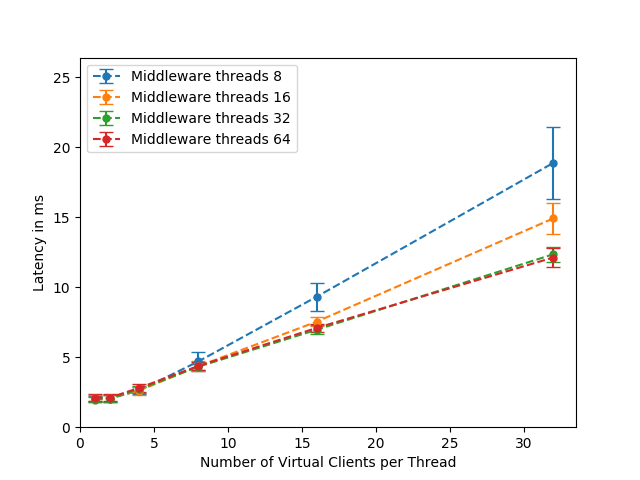
\includegraphics[width=\textwidth]{img/exp3_2/exp3_2__latency_client_write_1.png}
    \caption{Latency write only}
    \label{fig:mesh1}
\end{subfigure}%
\begin{subfigure}{.5\textwidth}
      \centering
    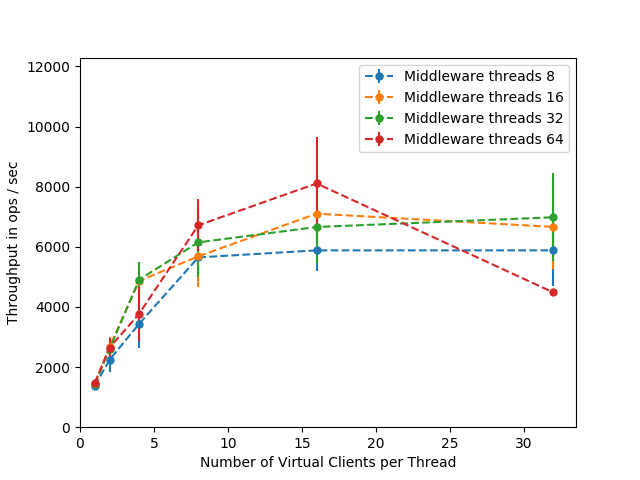
\includegraphics[width=\textwidth]{img/exp3_2/exp3_2__throughput_client_write_1.png}
    \caption{Throughput write only}
    \label{fig:mesh1}
\end{subfigure}
\caption{Exp3.2: Latency and throughputs as measures by the clients}
\label{fig:test}
\end{figure}

\subsubsection{Explanation}

I will now further elaborate the explanation from the above sections, using the some statistics including the average queuesize per configuration, and the time spent in each possible stage of the lifetime of a thread.

First of all, for read-only requests, the queuesize does increase as we have fewer numbers of middleware threads.
However, because saturation (from the server side) is reached quickly, this has no affect on the performance. 

For write-only requests, the queue-size is more interesting.
The queue is emptied much faster when as we increase the number of available middleware threads.
This emptying allows for a higher throughput, as more requests can be handled this way.
The right graph below supports this claim.
I will analyse the time of a request spent at each stage even further.

\begin{figure}[H]
\centering
\begin{subfigure}{.45\textwidth}
    \centering
    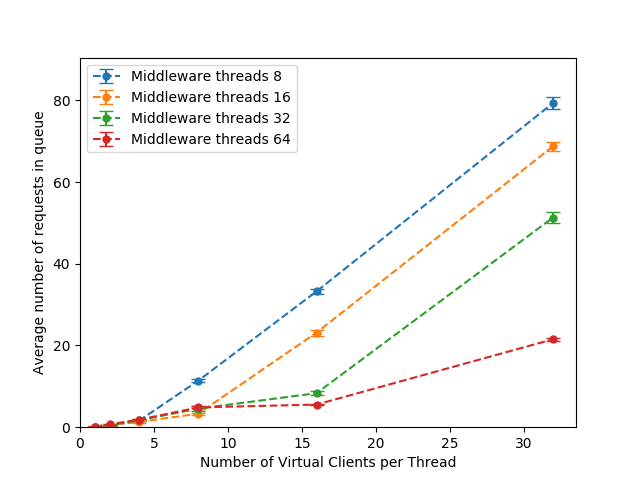
\includegraphics[width=\textwidth]{img/exp3_2/exp3_2__queuesize_middleware_write_0.png}
    \caption{Read-only}
    \label{fig:mesh1}
\end{subfigure}%
\begin{subfigure}{.45\textwidth}
      \centering
    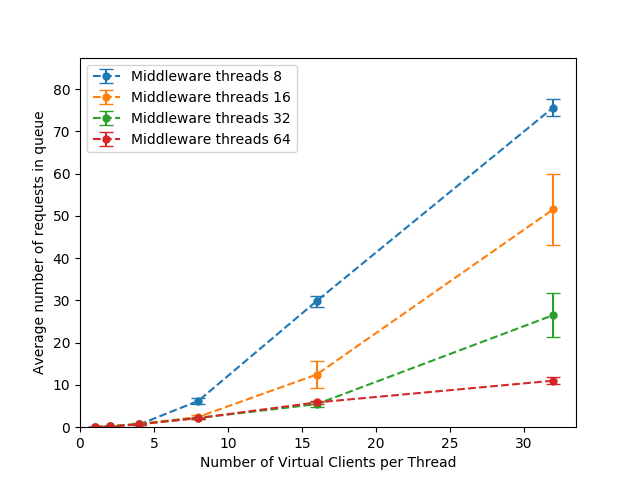
\includegraphics[width=\textwidth]{img/exp3_2/exp3_2__queuesize_middleware_write_1.png}
    \caption{Write-only}
    \label{fig:mesh1}
\end{subfigure}
\caption{Exp3.2: Average Queuesize in middleware \textbf{per} number of middleware threads and \textbf{per} virtual cliens per memtier thread}
\label{fig:test}
\end{figure}

%TODO : compare read-only and write-only operations 
%TODO more threads for 3.2 writes only, to check if saturation is reached (or what the maximum number is going to be?

The following plots allow for a more throughput analysis, supporting the explanations made in the previous subsection (subsection 3.2).
For a concise analysis, I only show the graphs for the two extreme configurations (virtual clients per memtier thread equals 1 , or equals 32).
For the other configurations, please view the appendix. \\
The claim we made before was that - for write-only requests - the number of middleware threads is the bottleneck, which implies that increasing this number lowers the waiting time in the queue.
The right figures in the following graph support this claim.
As more middleware threads are added, the relative time spent in the queue decreases compared to the waiting time (time spent to wait for servers response). 
The graph shows that for 32 virtual clients per memtier thread, the ratio is approximately $16 / 2 = 8$ for 8 middleware threads, whereas this ratio decreases to approximately $ 2 / 5 = 2.5 $ for 64 middleware threads.
This means much less times is spent in the queue itself, and simply waiting for the memcached server to respond.
One can also see, that the system is (as claimed before) not saturated with 1 virtual client.\\

\begin{figure}[H] 
  \label{ fig7} 
  \begin{minipage}[b]{0.45\linewidth}
    \centering
    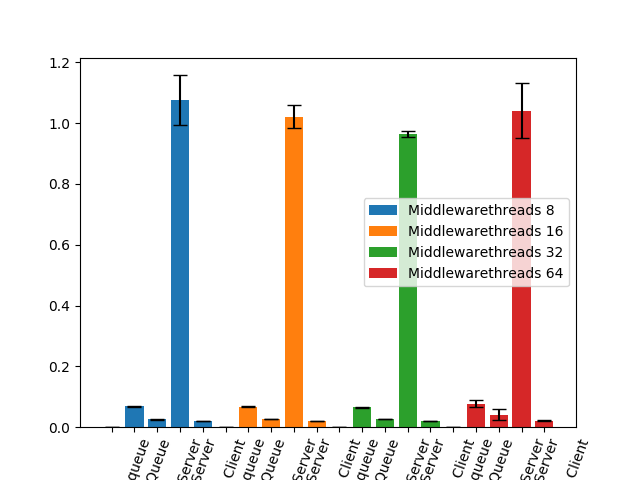
\includegraphics[width=0.7\linewidth]{img/exp3_2/exp3_2_mw_percentile_plots_writes_0__vc_1.png} 
    \caption{Read-only with 1 virtual client per memtier threads} 
    \vspace{4ex}
  \end{minipage}%%
  \begin{minipage}[b]{0.45\linewidth}
    \centering
    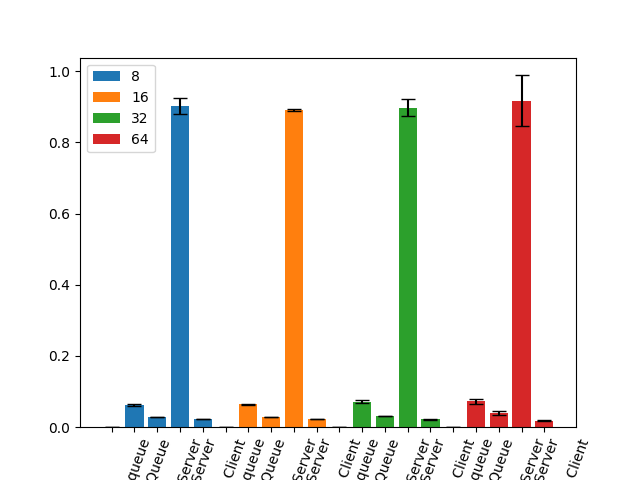
\includegraphics[width=0.7\linewidth]{img/exp3_2/exp3_2_mw_percentile_plots_writes_1__vc_1.png} 
    \caption{Read-only with 32 virtual client per memtier threads} 
    \vspace{4ex}
  \end{minipage} 
    \begin{minipage}[b]{0.45\linewidth}
    \centering
    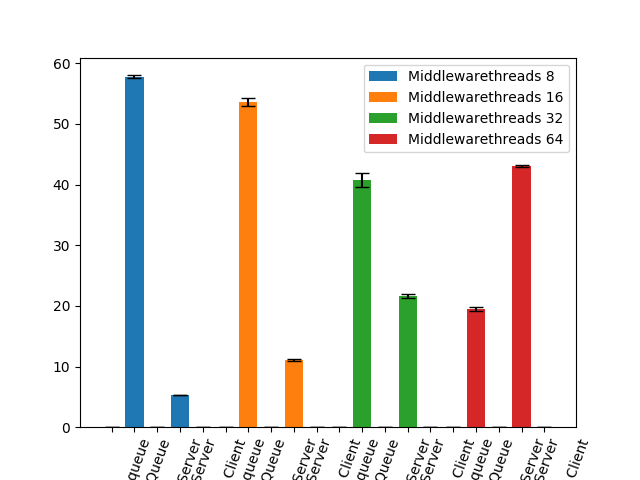
\includegraphics[width=0.7\linewidth]{img/exp3_2/exp3_2_mw_percentile_plots_writes_0__vc_32.png} 
    \caption{Write-only with 1 virtual client per memtier threads} 
    \vspace{4ex}
  \end{minipage}%% 
  \begin{minipage}[b]{0.45\linewidth}
    \centering
    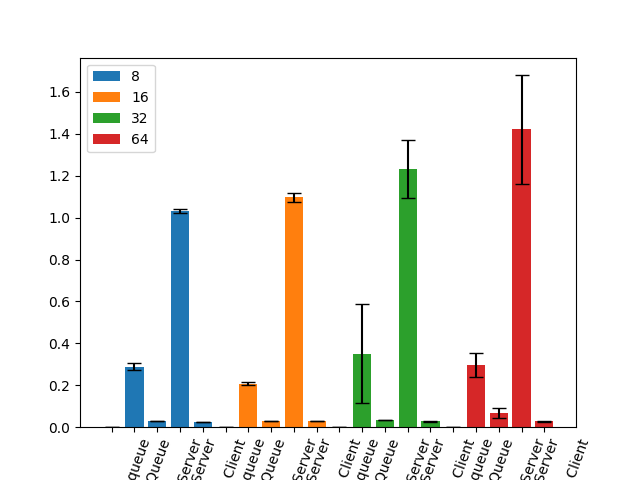
\includegraphics[width=0.7\linewidth]{img/exp3_2/exp3_2_mw_percentile_plots_writes_1__vc_32.png} 
    \caption{Write-only with 32 virtual client per memtier threads} 
    \vspace{4ex}
  \end{minipage} 
  \caption{Exp3.2: Time spent at different stages of the lifetime of a request. Each graph distinguished between read-only and write-only operations, as well as the number of virtual clients per memtier-thread (1 or 32)}
\end{figure}

\subsection{Summary}

\begin{center}
	{Maximum throughput for one middleware.}
	\begin{tabular}{|l|p{2cm}|p{2cm}|p{2cm}|p{2cm}|}
		\hline                                & Throughput & Response time & Average time in queue & Miss rate \\ 
		\hline Reads: Measured on middleware  & 3348 & 0.94 ms & 0.086 ms &           0 \\ 
		\hline Reads: Measured on clients     & 3321 & 1.81 ms & n/a                   &           0 \\ 
		\hline Writes: Measured on middleware & 7658 & 2.16 ms & 0.824 ms & n/a       \\ 
		\hline Writes: Measured on clients    & 7629 & 12.57 ms & n/a                   & n/a       \\ 
		\hline 
	\end{tabular}
\end{center}

\begin{center}
	{Maximum throughput for two middlewares.}
	\begin{tabular}{|l|p{2cm}|p{2cm}|p{2cm}|p{2cm}|}
		\hline                                & Throughput & Response time & Average time in queue & Miss rate \\ 
		\hline Reads: Measured on middleware  & 10330 & 31.40 &                       &           0\\ 
		\hline Reads: Measured on clients     & 11116 &  32.37 & n/a                   &           0\\ 
		\hline Writes: Measured on middleware & 8131 & 11.13 &                       & n/a       \\ 
		\hline Writes: Measured on clients    & 8108 & 14.27 & n/a                   & n/a       \\ 
		\hline 
	\end{tabular}
\end{center}

Notice that the miss rate is always zero, because this is 1. a closed system, and all servers are pre-populated before any experiment starts.

Based on the data provided in these tables, write at least two paragraphs summarizing your findings about the performance of the middleware in the baseline experiments. \\

Also, when having only one middleware, the middleware is the bottleneck.
This can be seen from comparing experiment 2.1 and recognising that for write-only operations, the exact same setup decreases from $18'000 ops/sec$ to $8'000 ops/sec$.
As such, adding the second middleware doubles this capacity, from $8'000 ops/sec$ to $16'000 ops/sec$, as we now have independelty two servers that can send out these requests.
The graphs of for write-only operations in section 2.1, and section 3.1 resp. section 3.2 underline these statements. \\

One can see this also from the fact that the middleware may not have enough middleware threads.
For 3.1 writes-only, the throughput plateaus at almost $8'000 ops/sec$ when we have 64 middleware-threads.
In 3.2 one can observer, that we now increase the number of middleware-threads to a total of $2 \times 64 = 128$ middlewarethreads (in the entire system). 
As a result, the throughput also almost doubles, and one cannot recognise a saturation phase.
This implies that adding more middleware-threads possibly could result at the original, almost $18'000 ops/sec$ calculation. \\

%TODO potentially make this experiment, with one middleware, and 128, and 256 threads? and check if this hypothesis is correct?

%TODO talk more about queue times, queue sizes etc.




\section{Throughput for Writes (90 pts)}

\subsection{Full System}
I am connecting three load generating client VMs to two middlewares.
These middlewares are connected to three memcached server VMs each.
I have the following setup.

\begin{center}
	\scriptsize{
		\begin{tabular}{|l|c|}
			\hline Number of servers                & 3          \\ 
			\hline Number of client machines        & 3          \\ 
			\hline Instances of memtier per machine & 2          \\ 
			\hline Threads per memtier instance     & 1          \\
			\hline Virtual clients per thread       & [1..32]    \\ 
			\hline Workload                         & Write-only \\
			\hline Number of middlewares            & 2          \\
			\hline Worker threads per middleware    & [8..64]    \\
			\hline Repetitions                      & 3 or more (at least 1 minute each)  \\ 
			\hline 
		\end{tabular}
	} 
\end{center}

During this experiment, I iterate over all possible permutations of virtual clients per thread (in the range of [1, 2, 4, 8, 16, 32]), and worker threads per middlewares (in the range of [8, 16, 32, 64]).
I run each experiment for 90 seconds (which includes a 15 second warm-up and a 15 second cool-down time). 
Each experiment again consists of three trials from which we measure the mean and the standard deviation.
This section only covers write-only experiments.
I cover response time (latency) , and throughput. \\

The following are graphs from the middleware.

\begin{figure}[H]
\centering
\begin{subfigure}{.5\textwidth}
    \centering
    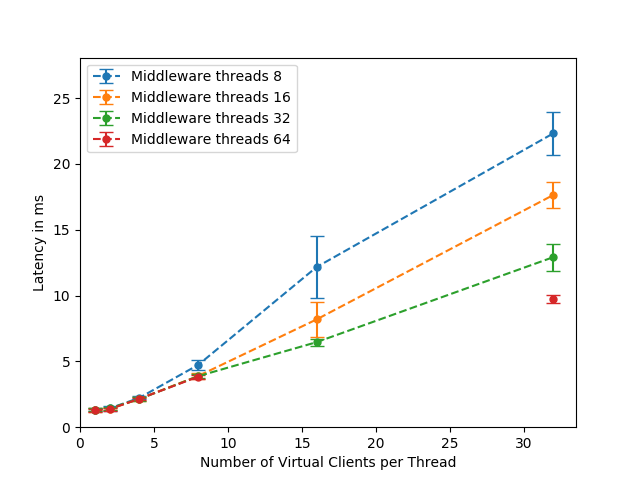
\includegraphics[width=\textwidth]{img/exp4_1/exp4_1__vc_64__latency_middleware_write_1.png}
    \caption{Latency write only}
    \label{fig:mesh1}
\end{subfigure}%
\begin{subfigure}{.5\textwidth}
      \centering
    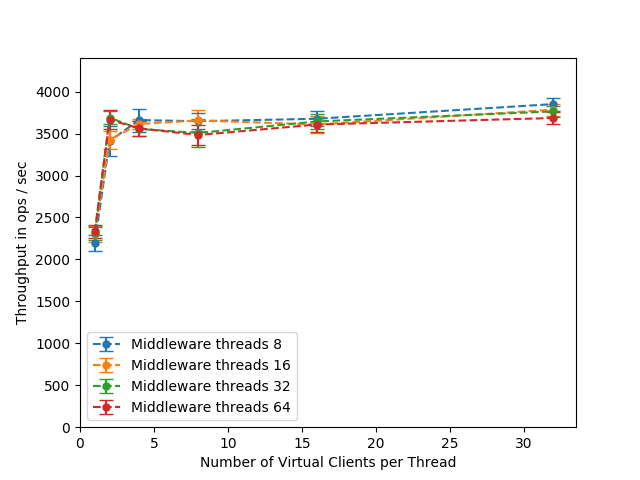
\includegraphics[width=\textwidth]{img/exp4_1/exp4_1__vc_64__throughput_middleware_write_1.png}
    \caption{Throughput write only}
    \label{fig:mesh1}
\end{subfigure}
\caption{Exp3.2: Latency and throughputs as measures by the middlewares}
\label{fig:test}
\end{figure}

\begin{figure}[H]
\centering
\begin{subfigure}{.5\textwidth}
    \centering
    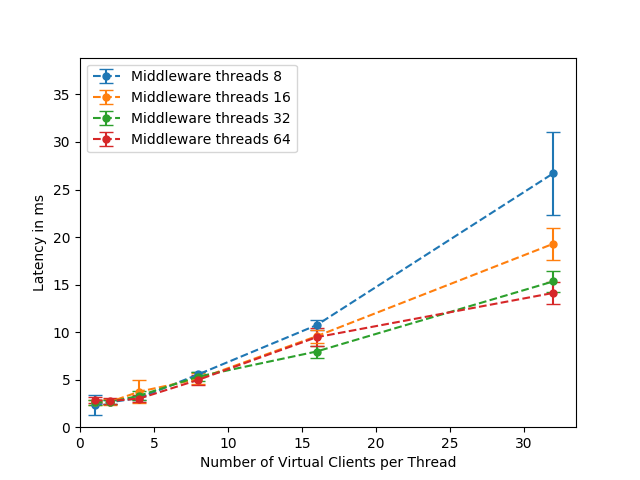
\includegraphics[width=\textwidth]{img/exp4_1/exp4_1__vc_64__latency_client_write_1.png}
    \caption{Latency write only}
    \label{fig:mesh1}
\end{subfigure}%
\begin{subfigure}{.5\textwidth}
      \centering
    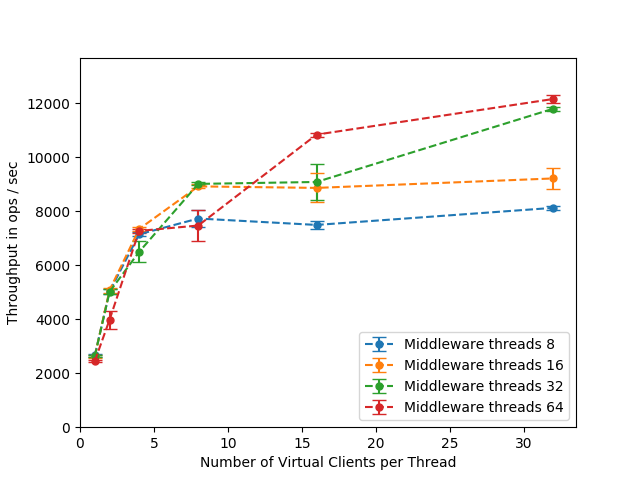
\includegraphics[width=\textwidth]{img/exp4_1/exp4_1__vc_64__throughput_client_write_1.png}
    \caption{Throughput write only}
    \label{fig:mesh1}
\end{subfigure}
\caption{Exp3.2: Latency and throughputs as measures by the clients}
\label{fig:test}
\end{figure}

\subsubsection{Explanation}

Provide a detailed analysis of the results (e.g., bottleneck analysis, component utilizations, average queue lengths, system saturation). Add any additional figures and experiments that help you illustrate your point and support your claims.


\begin{figure}[H]
\centering
\begin{subfigure}{.5\textwidth}
      \centering
    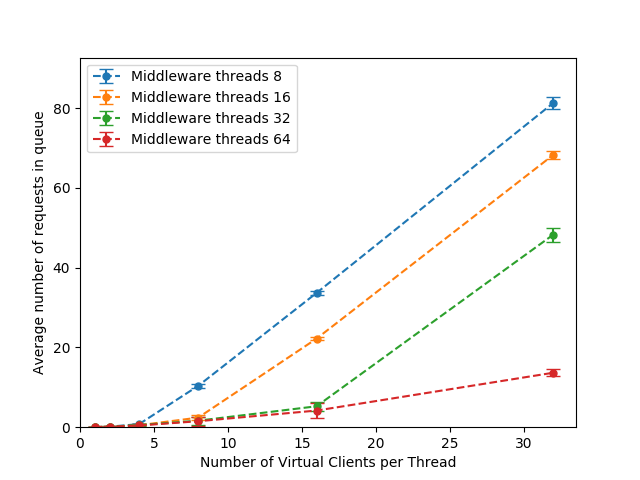
\includegraphics[width=\textwidth]{img/exp4_1/exp4_1__queuesize_middleware_write_1.png}
    \caption{Throughput read only}
    \label{fig:mesh1}
\end{subfigure}
\caption{Exp3.1: Latency and throughputs as measures by the \textbf{middlewares}}
\label{fig:test}
\end{figure}

%TODO : compare read-only and write-only operations 
%TODO measure system saturation with dstat? i.e. if 100% at 8 VC and at 32 VC?
%TODO talk about respective response times

%TODO more threads for 3.2 writes only, to check if saturation is reached (or what the maximum number is going to be?

\begin{figure}[H] 
  \label{ fig7} 
  \begin{minipage}[b]{0.5\linewidth}
    \centering
    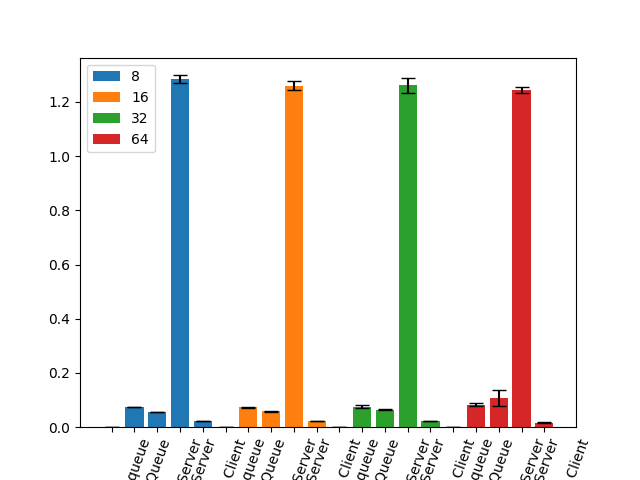
\includegraphics[width=0.7\linewidth]{img/exp4_1/exp4_1_mw_percentile_plots_writes_1__vc_1.png} 
    \caption{Initial condition} 
    \vspace{4ex}
  \end{minipage}%%
  \begin{minipage}[b]{0.5\linewidth}
    \centering
    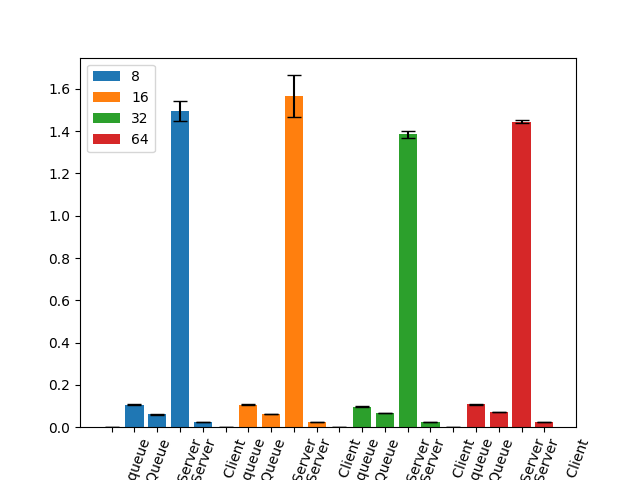
\includegraphics[width=0.7\linewidth]{img/exp4_1/exp4_1_mw_percentile_plots_writes_1__vc_2.png} 
    \caption{Rupture} 
    \vspace{4ex}
  \end{minipage} 
  \begin{minipage}[b]{0.5\linewidth}
    \centering
    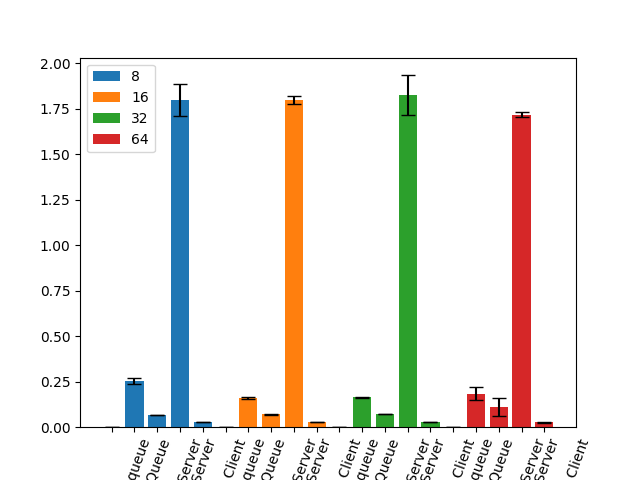
\includegraphics[width=0.7\linewidth]{img/exp4_1/exp4_1_mw_percentile_plots_writes_1__vc_4.png} 
    \caption{DFT, Initial condition} 
    \vspace{4ex}
  \end{minipage}%% 
  \begin{minipage}[b]{0.5\linewidth}
    \centering
    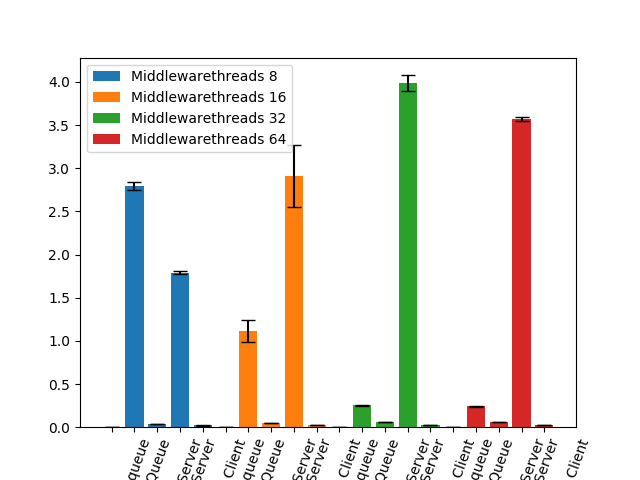
\includegraphics[width=0.7\linewidth]{img/exp4_1/exp4_1_mw_percentile_plots_writes_1__vc_8.png} 
    \caption{DFT, rupture} 
    \vspace{4ex}
  \end{minipage} 
    \begin{minipage}[b]{0.5\linewidth}
    \centering
    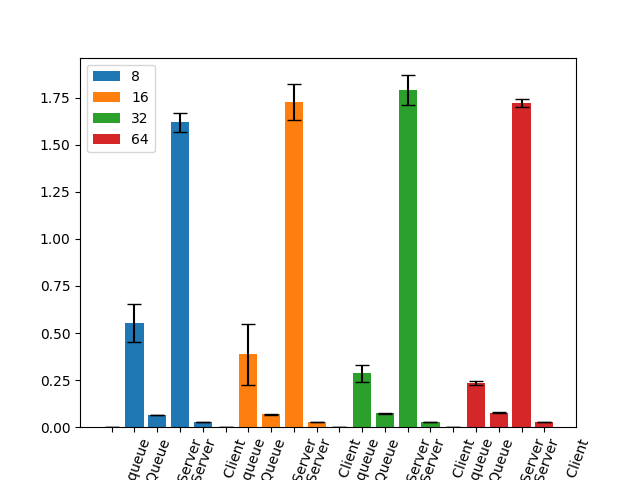
\includegraphics[width=0.7\linewidth]{img/exp4_1/exp4_1_mw_percentile_plots_writes_1__vc_16.png} 
    \caption{DFT, Initial condition} 
    \vspace{4ex}
  \end{minipage}%% 
  \begin{minipage}[b]{0.5\linewidth}
    \centering
    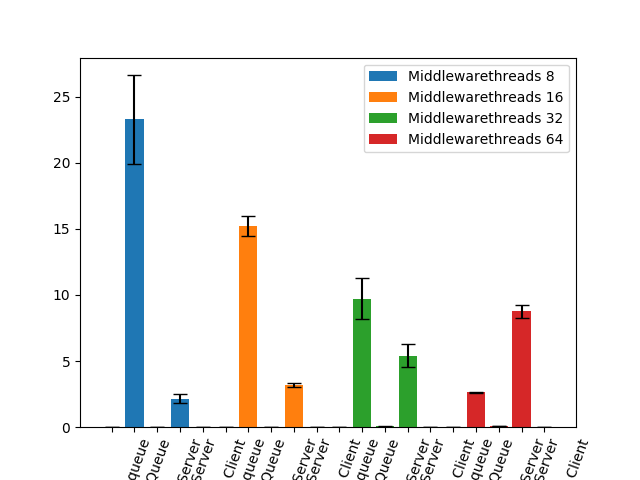
\includegraphics[width=0.7\linewidth]{img/exp4_1/exp4_1_mw_percentile_plots_writes_1__vc_32.png} 
    \caption{DFT, rupture} 
    \vspace{4ex}
  \end{minipage} 
    \begin{minipage}[b]{0.5\linewidth}
    \centering
    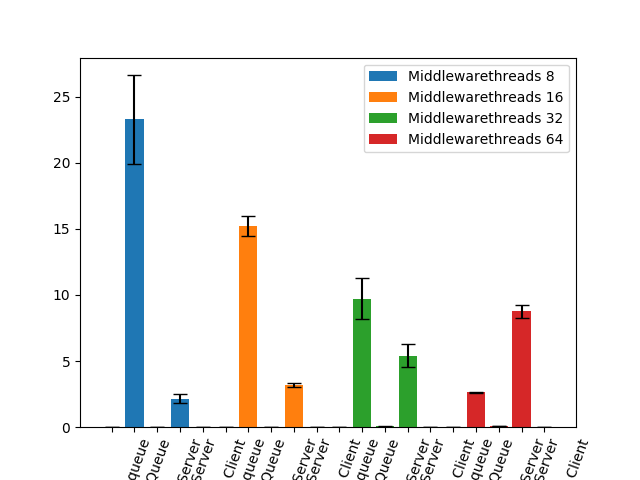
\includegraphics[width=0.7\linewidth]{img/exp4_1/exp4_1_mw_percentile_plots_writes_1__vc_32.png} 
    \caption{DFT, Initial condition} 
    \vspace{4ex}
  \end{minipage}%% 
  \begin{minipage}[b]{0.5\linewidth}
    \centering
    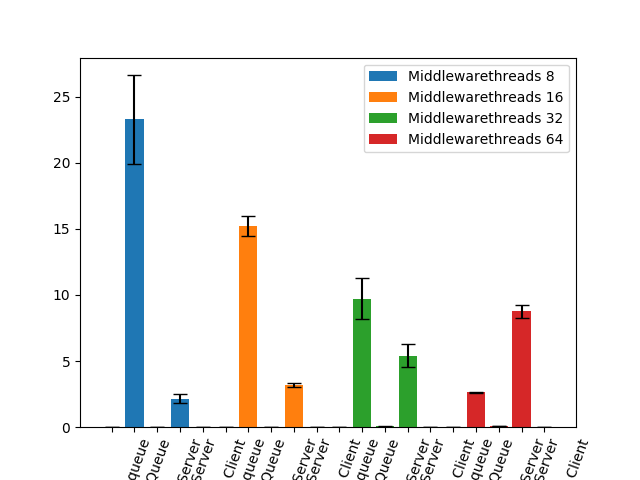
\includegraphics[width=0.7\linewidth]{img/exp4_1/exp4_1_mw_percentile_plots_writes_1__vc_32.png} 
    \caption{DFT, rupture} 
    \vspace{4ex}
  \end{minipage} 
\end{figure}

\subsection{Summary}

Based on the experiments above, fill out the following table with the data corresponding to the maximum throughput point for all four worker-thread scenarios.

\begin{center}
	{Maximum throughput for the full system}
	\begin{tabular}{|l|p{1.5cm}|p{1.5cm}|p{1.5cm}|p{1.5cm}|}
		\hline                                            & WT=8 & WT=16 & WT=32 & WT=64 \\ 
		\hline Throughput (Middleware)                    & 14365 & 18338 & 18828 & 17984 \\ 
		\hline Throughput (Derived from MW response time) & 14632 & 18827 & 18504 & 17830  \\ 
		\hline Throughput (Client)                     &14858 & 17017 & 15703 & 17503 \\ 
		\hline Average time in queue                      &      &       &       &       \\ 
		\hline Average length of queue                    &      &       &       &       \\ 
		\hline Average time waiting for memcached         &      &       &       &       \\ 
		\hline 
	\end{tabular}
\end{center}

Based on the data provided in these tables, draw conclusions on the state of your system for a variable number of worker threads.

\section{Gets and Multi-gets (90 pts)}

I use three load generating machines, two middlewares and three memcached servers. Each memtier instance has 2 virtual clients in total and the number of middleware worker threads is 64, as determined by previous experiments, providing the highest throughput.

For multi-GET workloads, I use the \texttt{--ratio} parameter to specify the exact ratio between SETs and GETs. I measure response time on the client as a function of multi-get size, with and without sharding on the middlewares.

\subsection{Sharded Case}

I run multi-gets with 1, 3, 6 and 9 keys (memtier configuration) with sharding enabled (multi-gets are broken up into smaller multi-gets and spread across servers). 
The following describes the detailed experiment setup.

\begin{center}
	\scriptsize{
		\begin{tabular}{|l|c|}
			\hline Number of servers                & 3                       \\ 
			\hline Number of client machines        & 3                       \\ 
			\hline Instances of memtier per machine & 2                       \\ 
			\hline Threads per memtier instance     & 1                       \\
			\hline Virtual clients per thread       & 2     		            \\ 
			\hline Workload                         & ratio=1:$<$Multi-Get size$>$             \\
			\hline Multi-Get behavior               & Sharded                 \\
			\hline Multi-Get size                   & [1..9]                  \\
			\hline Number of middlewares            & 2                       \\
			\hline Worker threads per middleware    & max. throughput config. \\
			\hline Repetitions                      & 3 or more (at least 1 minute each)               \\ 
			\hline 
		\end{tabular}
	} 
\end{center}

The following are average response time as measured on the client, as well as the 25th, 50th, 75th, 90th and 99th percentiles.

To double-check that the above graph is correct (mainly the averages of the individual keysizes), I analyse the response time and throughput graphs.
I will only include graphs from the middleware as these values don't include the warm-up and the cool-down times.
However, the values measured as per client do conform with the trends found in the graph. 

\begin{figure}[H]
\centering
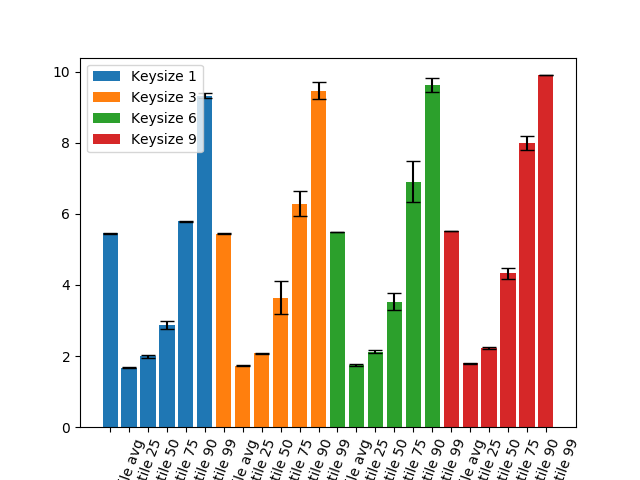
\includegraphics[width=\textwidth]{img/exp5_1/exp5_1_client_percentile_plots_sharded_True.png}
\caption{Exp3.2: Latency and throughputs as measures by the middlewares}
\label{fig:test}
\end{figure}

The multiegets all have a similar response time.
This is because the middleware does not internally distinguish between sending only a single packet, and multiple packets to the servers, as long as these packets fully fit into the \textit{byteBuffer}.
As my byteBuffer is of size $20 * 1024 * 4$, and a single "full" datapacket for message is of size $ 4096 $, this easily fits into the byteBuffer.
As such, there is no significant slowdown in the response time.
However, because of the higher memory requirements, bigger multi-gets tend to be a bit more unstable (as this requires more operations, and more operations can cause delays).
This can be seen in the graph, where the latency percentiles (especially the 90th percentiles) increase with a higher number of keysizes. \\

To do a sanity check, I include the total latency and throughputs as measured by the clients (because the above histogram was derived from client values).
One can clearly see that the trend presented in the above barchart is supported by the response times measured by the clients.
In additional to that, the inverse law for throughput and latency holds, as the throughput and latency both have an overall almost constant tendency (with the exception of the keysize "9" decreasing throughput slightly, and increasing the latency slightly).

\begin{figure}[H]
\centering
\begin{subfigure}{.5\textwidth}
    \centering
    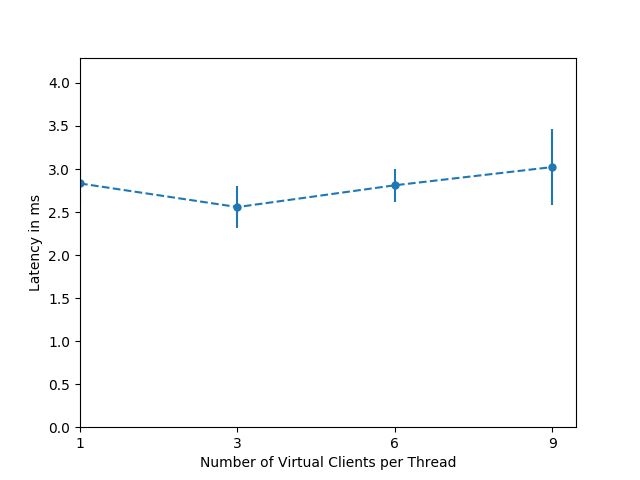
\includegraphics[width=\textwidth]{img/exp5_1/exp5_1__client_latency_sharding_True.png}
    \caption{Latency write only}
    \label{fig:mesh1}
\end{subfigure}%
\begin{subfigure}{.5\textwidth}
      \centering
    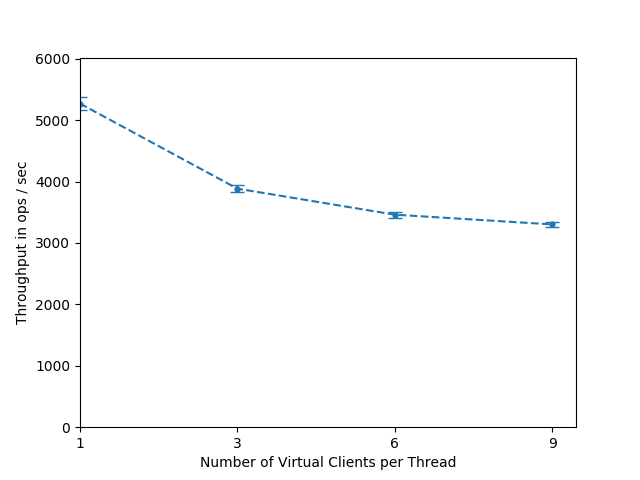
\includegraphics[width=\textwidth]{img/exp5_1/exp5_1__client_throughput_sharding_True.png}
    \caption{Throughput write only}
    \label{fig:mesh1}
\end{subfigure}
\caption{Exp3.2: Latency and throughputs as measures by the clients}
\label{fig:test}
\end{figure}


As a sanity check, the interactive applies, which means that the latency increases when the throughput decreases.
As one can see, the graphs support this claim of the inverse correlation between response time and throughput.

\subsubsection{Explanation}

The bottleneck is either the server which has to respond to all the get-requests (and can do some compoundedly in the case of multi-gets with keysize > 1), or the middleware which does not allow the client to push more requests towards the server.
However, because the bandwidth of the middleware is so high, and theoretically supports almost $35'000 ops/sec$, it is highly likely that it is again the servers which cannot utilize more than the existing bandwidth of $3'000 ops/sec$.
This relates to experiment 2.2 (baseline no middleware, read-only), where one single client instance is able to max out the servers fairly quickly. 
The latency caused by contacting multiple servers instead of just one can be seen by comparing these values to the non-sharded case.
However, this network overhead is negligible as can be seen by comparing the graphs for the sharded case, vs. for the non-sharded case.
\\

However, it could also be the middleware which is not able to pass on all requests quick enough.
This would also explain the drop from $ 6'000 ops/sec $ in experiment 2.2, to $ 3'500 ops/sec$ in this experiment.
After doing a profiling of the code, I recognize that the java function \textbf{String.split} takes up most of the performance, and heavily increases system utilization.

%TODO  average queue length over time! system saturation?

\subsection{Non-sharded Case}

I run multi-gets with 1, 3, 6 and 9 keys (memtier configuration) with sharding disabled. 
The following provides a more detailed view of the configuration that I used.

\begin{center}
	\scriptsize{
		\begin{tabular}{|l|c|}
			\hline Number of servers                & 3                       \\ 
			\hline Number of client machines        & 3                       \\ 
			\hline Instances of memtier per machine & 2                       \\ 
			\hline Threads per memtier instance     & 1                       \\
			\hline Virtual clients per thread       & 2                		 \\ 
			\hline Workload                         & ratio=1:$<$Multi-Get size$>$              \\
			\hline Multi-Get behavior               & Non-Sharded             \\
			\hline Multi-Get size                   & [1..9]                  \\
			\hline Number of middlewares            & 2                       \\
			\hline Worker threads per middleware    & max. throughput config. \\
			\hline Repetitions                      & 3 or more (at least 1 minute each)               \\ 
			\hline 
		\end{tabular}
	} 
\end{center}

I plot average response time as measured on the client, as well as the 25th, 50th, 75th, 90th and 99th percentiles.

\begin{figure}[H]
\centering
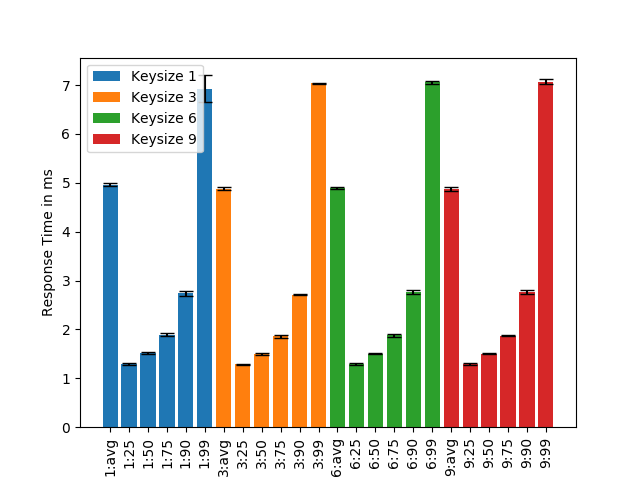
\includegraphics[width=\textwidth]{img/exp5_1/exp5_1_client_percentile_plots_sharded_False.png}
\caption{Exp3.2: Latency and throughputs as measures by the middlewares}
\label{fig:test}
\end{figure}

Internally and inside the middleware, the non-sharded multiegets are treated exactly like multigets with keysize 1.
This means - if the middleware operates well - that the response time and throughput should be very similar for any of the presented multiget keysize values.
And this is indeed the case. 
The average and percentiles match up in response time as can be seen from the graph.
There are some deviations, but these deviations are all within the error bounds of the other multikey-get sizes.
The reason behind the very similar multi-key-getsizes is also the \textit{byteBuffer} that I use, which allows each multikey-get request to fit into the buffer.
As my byteBuffer is of size $20 * 1024 * 4$, and a single "full" datapacket for message is of size $ 4096 $, this easily fits into the byteBuffer.
As such, there is no statistically significant decrease or increase in the response time or throughput. \\

To do a sanity check, I include the total latency and throughputs as measured by the clients (because the above histogram was derived from client values).
One can clearly see that the trend presented in the above barchart is supported by the response times measured by the clients.
In additional to that, the inverse law for throughput and latency holds, as the throughput and latency both have an overall almost constant tendency (with the exception of the keysize "9" decreasing throughput slightly, and increasing the latency slightly).

To double-check that the above graph is correct (mainly the averages of the individual keysizes), I analyse the response time and throughput graphs.
I will only include graphs from the middleware as these values don't include the warm-up and the cool-down times.
However, the values measured as per client do conform with the trends found in the graph. 

\begin{figure}[H]
\centering
\begin{subfigure}{.5\textwidth}
    \centering
    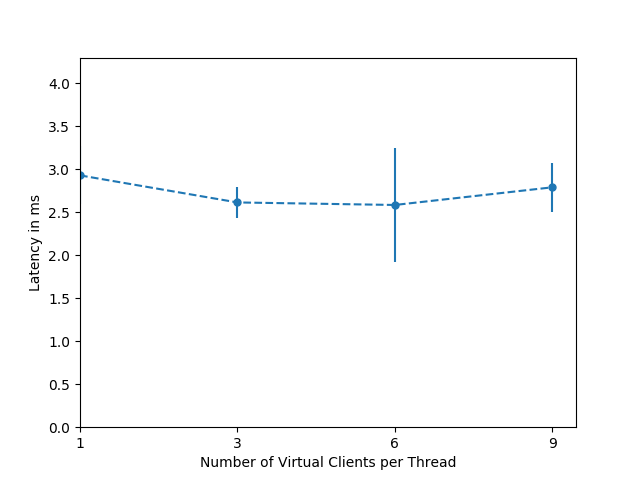
\includegraphics[width=\textwidth]{img/exp5_1/exp5_1__client_latency_sharding_False.png}
    \caption{Latency write only}
    \label{fig:mesh1}
\end{subfigure}%
\begin{subfigure}{.5\textwidth}
      \centering
    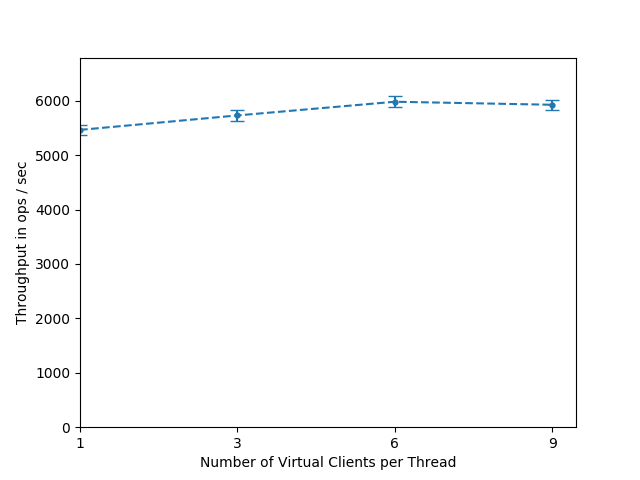
\includegraphics[width=\textwidth]{img/exp5_1/exp5_1__client_throughput_sharding_False.png}
    \caption{Throughput write only}
    \label{fig:mesh1}
\end{subfigure}
\caption{Exp3.2: Latency and throughputs as measures by the clients}
\label{fig:test}
\end{figure}

As a sanity check, the interactive applies, which means that the latency increases when the throughput decreases.
As one can see, the graphs support this claim of the inverse correlation between response time and throughput.

%TODO  average queue length over time! system saturation?
%TODO  code profiling?

\subsubsection{Explanation}

Provide a detailed analysis of the results (e.g., bottleneck analysis, component utilizations, average queue lengths, system saturation). Add any additional figures and experiments that help you illustrate your point and support your claims.

\subsection{Histogram}

For the case with 6 keys inside the multi-get, I now display four histograms representing the sharded and non-sharded response time distribution, both as measured on the client, and inside the middleware. 
I chose the bucket sizes such that the represent intervals of at least 100 micro-seconds (i.e. 1/10th of a millisecond).
After considering taking the mean of multiple items, I arrived at the conclusion of only picking a single memtier-instance's output and plotting this. 
This is for two reasons. 
1. This gives us a more true distribution, and not a flattened mean. Furthermore this is a good approximation, because all latency-histograms (across all memtier-instances) are very similarly distributed.
2. Adding multiple histograms together which are slightly deviated on the x-axis will increase the common latencies (around 2 milliseconds), and proportionally decrease the flatter regions, which also provide information to the reader.
By just picking one instance, I solve this problem and allow for a clearer display of these flat regions (also because the spikes are clearly visible in either case).

\begin{figure}[H]
\centering
\begin{subfigure}{.5\textwidth}
    \centering
    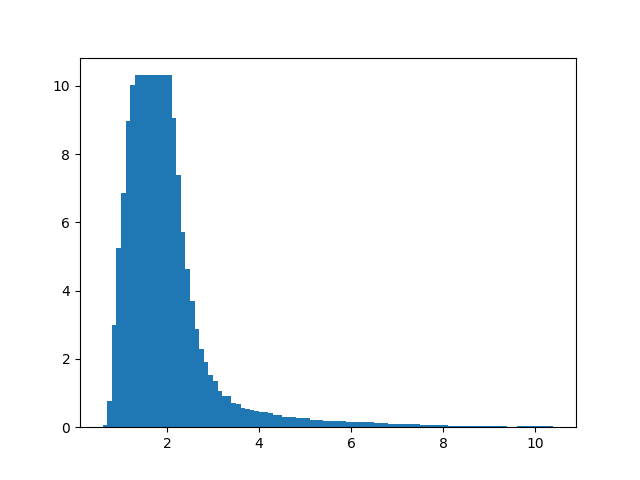
\includegraphics[width=\textwidth]{img/exp5_1/histogram_client_nonsharded.png}
    \caption{Non-Sharded Latency Histogram}
    \label{fig:mesh1}
\end{subfigure}%
\begin{subfigure}{.5\textwidth}
      \centering
    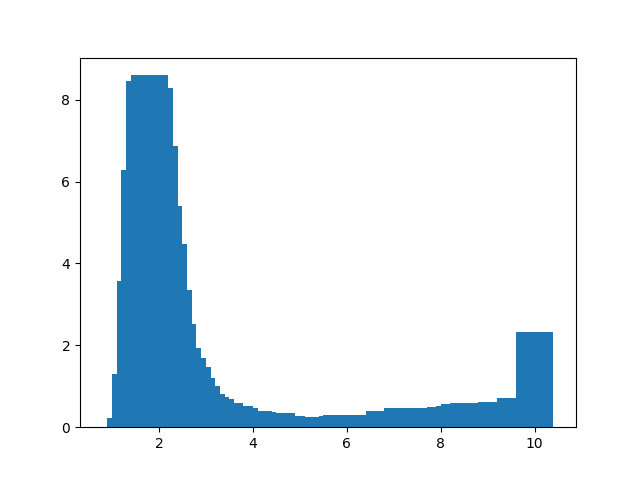
\includegraphics[width=\textwidth]{img/exp5_1/histogram_client_sharded.png}
    \caption{Sharded Latency Histogram}
    \label{fig:mesh1}
\end{subfigure}
\caption{Exp3.2: Latency and throughputs as measures by the clients}
\label{fig:test}
\end{figure}

%TODO fix displaying the 

More network operations come from the fact that more individual servers need to be contact to finish a request (instead of one server, all servers need to be communicated with).
This can be seen in the histogram because the sharded case has a longer tail, as this requires 1. more operations (i.e. more computation effort), as was measured using the tool dstat, and 2. requires more network operations. \\

The client includes the network round-trip between sending it off from the client machine, and arriving at the middleware.
In contrast, the middleware only views latency as the round-trip time from incoming request (right before entering the queue), and right before sending the response back to the client.
This can be seen in the graphs, as the middleware histograms are shifter to the left w.r.t. the client histograms.


\subsection{Summary}

Provide a detailed comparison of the sharded and non-shareded modes. For which multi-GET size is sharding the preferred option? Provide a detailed analysis of your system. Add any additional figures and experiments that help you illustrate your point and support your claims.

\section{2K Analysis (90 pts)}

This 2k analysis includes the analysis of any correlations between the following factors: 1. number of memcached servers, 2. the number of middleware vm's and finally 3. the number of worker threads per middleware.
The following table shows which possible values we cross-reference, such that we can later on analyse which factors have the most impact on throughput and response time.

\begin{itemize}
		
	\item Memcached servers: 1 and 3
	\item Middlewares: 1 and 2
	\item Worker threads per MW: 8 and 32
	      	      
\end{itemize}


Any configuration is run 3 times (3 repetitions) for 90 seconds, which implies a 15 second warm-up and a 15 second cool-down time.
The following table shows a detailed configuration of my setup.

\begin{center}
	\scriptsize{
		\begin{tabular}{|l|c|}
			\hline Number of servers                & 1 and 3                                     \\ 
			\hline Number of client machines        & 3                                           \\ 
			\hline Instances of memtier per machine & 1 (1 middleware) or 2 (2 middlewares) \\ 
			\hline Threads per memtier instance     & 2 (1 middleware) or 1 (2 middlewares)   \\
			\hline Virtual clients per thread       &  32                                     \\ 
			\hline Workload                         & Write-only and Read-only\\
			\hline Number of middlewares            & 1 and 2                                     \\
			\hline Worker threads per middleware    & 8 and 32                                    \\
			\hline Repetitions                      & 3 or more (at least 1 minute each)                                   \\ 
			\hline 
		\end{tabular}
	} 
\end{center}

I apply this analysis once for read-only workloads, and then separately for write-only workloads, as both procedures are fundamentally different.
I don't use any multi-get behavior (i.e. keysize is always 1 for read-only workloads). \\

For read-only and work-only workloads, I created tables which represent all possible configurations.
For both subsections, I will use the following abbreviations (and variable-names)

\begin{itemize}
\item NS: Number of Servers
\item NM: Number of Middlewares
\item WTMW: Worker threads per middleware
\end{itemize}

\subsubsection{Read-only}

% & Mean Latency 

\begin{center}
    \begin{tabular}{ | l | l | l | p{5cm} |}
    \hline
    NS (Servers) & NM (Middlewares) & WTMW (Workerthreads) & Mean Throughput \\ \hline
    1 & 1 & 8 & \\ \hline
    1& 1 & 32 & \\ \hline
    1 & 2 & 8 &  \\ \hline
   	1 & 2 & 32 & \\ \hline
    3 & 1 & 8 & \\ \hline
    3 & 1 & 32 &  \\ \hline
    3 & 2 & 8 &  \\ \hline
    3 & 2 & 32 &  \\
    \hline
    \end{tabular}
\end{center}

Repeat the experiment for (a)~a write-only and (b)~a read-only workload.
For each of the two workloads, what is the impact of these parameters on throughput, respectively response time?




\subsubsection{Write-only}



\section{Queuing Model (90 pts)}

In this section I model the workerqueue of the middleware (after the requests come in) using queueing theory to model how the system behaves with an asymptotically increasing number of threads.
In both subsection I will go use the different number of middleware (specifically, one of [8, 16, 32, 64]) threads to apply this analysis. \\

I choose the following input parameters to model the system:

\begin{enumerate}
\item Mean arrival rate $\lambda$: I choose the mean arrival rate by the number of virtual clients per memtier thread.
This rate is given by the \textbf{throughput as measured by the client-side in ops/sec}.
\item Mean service rate $\mu$: For the M/M/1 case, I choose the mean service rate to be the \textbf{maximum throughput which can possibly be handled by the middleware} within the configuration in section 4.
This means that I will choose the maximum possible throughput that the middleware experiences.
\end{enumerate}

%TODO why do you choose it like this?

The following table provides a quick reference to these values.
as given by the maximum throughput of the middleware (ops/sec) 
as given by the maximum throughput of the clients (ops/sec) 

\begin{center}
	\scriptsize{
		\begin{tabular}{|l|c|c|}
			\hline Threads in the middleware & 
			$\mu$ Service rate &
			$\lambda$ Arrival rate \\ 
			\hline 8 &   8278 & 8120 \\ 
			\hline 16 &  10491 & 9209 \\ 
			\hline 32 &  11775 & 11789 \\
			\hline 64 &  12984 & 12150 \\
			\hline
		\end{tabular}
	} 
\end{center}



\subsection{M/M/1}
In this subsection I model the behavior of the middleware and it's workerqueue using a M/M/1 queueing model. \\

I will predict the traffic intensity, the queue length, the latency and the wait time.
I will then compare these to the observed values from section 4.1 to arrive at a conclusion if the comparison makes sense.
The system is stable, as is specified by all the rho values which are all smaller than 1.

\begin{table}[H]
	\caption{M/M/1 Predicted vs. Observed values for 8 Middlewarethreads}
	\scriptsize{
		\begin{tabular}{|l|c|c|c|c|c|c|c|c|c|c|}
					\hline & & & Predicted & Predicted & Predicted & Observed & Observed & Observed &\\ 
			\hline Middelware threads $\mu$ & $\lambda$ & $\rho$ & Queue length & Latency & Wait time & Queue length & Latency & Wait time \\ 
			\hline 8 & 8278 & 8120 & 0.9809023 & 50.38 & 0.00632536 & 0.00620456 &  14365.88 \\ 
			\hline 16 & 10491 & 9209 & 0.87780868 & 6.31 & 0.00078007 & 0.00068475 &  14365.88 \\ 
			\hline 32 & 11810 & 11789 & 0.99885762 & 1796.46 & 0.15272627 & 0.15264135 &  14365.88 \\ 
			\hline 64 & 12984 & 12150 & 0.93577961 & 13.63 & 0.00119927 & 0.00112226 &  14365.88 \\ 
			\hline
		\end{tabular}
	} 
\end{table}

For each configuration of workerthreads, I will proceed with this calculation.


your entire system. Motivate your choice of input parameters to the model. Explain for which experiments the predictions of the model match and for which they do not.

\subsection{M/M/m}


\begin{table}[H]
	\caption{M/M/1 Predicted vs. Observed values for 8 Middlewarethreads}
	\scriptsize{
		\begin{tabular}{|l|c|c|c|c|c|c|c|c|c|c|}
					\hline & & & Predicted & Predicted & Predicted & Observed & Observed & Observed &\\ 
			\hline Middelware threads $\mu$ & $\lambda$ & $\rho$ & Queue length & Latency & Wait time & Queue length & Latency & Wait time \\ 
			\hline 8 & 1034 & 8120 & 0.9809023 & 50.38 & 0.00632536 & 0.00620456 &  14365.88 \\ 
			\hline 16 & 655 & 9209 & 0.87780868 & 6.31 & 0.00078007 & 0.00068475 &  14365.88 \\ 
			\hline 32 & 367 & 11789 & 0.99944397 & 1796.46 & 0.15272627 & 0.15264135 &  14365.88 \\ 
			\hline 64 & 202 & 12150 & 0.93577961 & 13.63 & 0.00119927 & 0.00112226 &  14365.88 \\ 
			\hline
		\end{tabular}
	} 
\end{table}

Build an M/M/m model based on Section 4, where each middleware worker thread is represented as one service.  Motivate your choice of input parameters to the model. Explain for which experiments the predictions of the model match and for which they do not.

\subsection{Network of Queues}

Based on Section 3, build a network of queues which simulates your system. Motivate the design of your network of queues and relate it wherever possible to a component of your system. Motivate your choice of input parameters for the different queues inside the network. Perform a detailed analysis of the utilization of each component and clearly state what the bottleneck of your system is. Explain for which experiments the predictions of the model match and for which they do not.

\section{Appendix}

\subsection{Experiment 3.1 - Baseline with one middleware}
For read-only experiments, I have the following throughput and response graph derivated from the values of the client:

\begin{figure}[!ht] 
  \label{ fig7} 
  \begin{minipage}[b]{0.5\linewidth}
    \centering
    \includegraphics[width=0.7\linewidth]{img/exp3_1/exp3_1_mw_percentile_plots_writes_0__vc_1.png} 
    \caption{Initial condition} 
    \vspace{4ex}
  \end{minipage}%%
  \begin{minipage}[b]{0.5\linewidth}
    \centering
    \includegraphics[width=0.7\linewidth]{img/exp3_1/exp3_1_mw_percentile_plots_writes_1__vc_1.png} 
    \caption{Rupture} 
    \vspace{4ex}
  \end{minipage} 
    \begin{minipage}[b]{0.5\linewidth}
    \centering
    \includegraphics[width=0.7\linewidth]{img/exp3_1/exp3_1_mw_percentile_plots_writes_0__vc_2.png} 
    \caption{Initial condition} 
    \vspace{4ex}
  \end{minipage}%%
  \begin{minipage}[b]{0.5\linewidth}
    \centering
    \includegraphics[width=0.7\linewidth]{img/exp3_1/exp3_1_mw_percentile_plots_writes_1__vc_2.png} 
    \caption{Rupture} 
    \vspace{4ex}
  \end{minipage} 
  \begin{minipage}[b]{0.5\linewidth}
    \centering
    \includegraphics[width=0.7\linewidth]{img/exp3_1/exp3_1_mw_percentile_plots_writes_0__vc_4.png} 
    \caption{DFT, Initial condition} 
    \vspace{4ex}
  \end{minipage}%% 
  \begin{minipage}[b]{0.5\linewidth}
    \centering
    \includegraphics[width=0.7\linewidth]{img/exp3_1/exp3_1_mw_percentile_plots_writes_1__vc_4.png} 
    \caption{DFT, rupture} 
    \vspace{4ex}
  \end{minipage} 
    \begin{minipage}[b]{0.5\linewidth}
    \centering
    \includegraphics[width=0.7\linewidth]{img/exp3_1/exp3_1_mw_percentile_plots_writes_1__vc_8.png} 
    \caption{DFT, rupture} 
    \vspace{4ex}
  \end{minipage} 
    \begin{minipage}[b]{0.5\linewidth}
    \centering
    \includegraphics[width=0.7\linewidth]{img/exp3_1/exp3_1_mw_percentile_plots_writes_1__vc_8.png} 
    \caption{DFT, rupture} 
    \vspace{4ex}
  \end{minipage} 
    \begin{minipage}[b]{0.5\linewidth}
    \centering
    \includegraphics[width=0.7\linewidth]{img/exp3_1/exp3_1_mw_percentile_plots_writes_0__vc_16.png} 
    \caption{DFT, Initial condition} 
    \vspace{4ex}
  \end{minipage}%% 
  \begin{minipage}[b]{0.5\linewidth}
    \centering
    \includegraphics[width=0.7\linewidth]{img/exp3_1/exp3_1_mw_percentile_plots_writes_1__vc_16.png} 
    \caption{DFT, rupture} 
    \vspace{4ex}
  \end{minipage} 
    \begin{minipage}[b]{0.5\linewidth}
    \centering
    \includegraphics[width=0.7\linewidth]{img/exp3_1/exp3_1_mw_percentile_plots_writes_0__vc_32.png} 
    \caption{DFT, Initial condition} 
    \vspace{4ex}
  \end{minipage}%% 
  \begin{minipage}[b]{0.5\linewidth}
    \centering
    \includegraphics[width=0.7\linewidth]{img/exp3_1/exp3_1_mw_percentile_plots_writes_1__vc_32.png} 
    \caption{DFT, rupture} 
    \vspace{4ex}
  \end{minipage} 
\end{figure}

\subsection{Experiment 3.2}
Here is the extensive bar-plot on where most time is spent:


\begin{figure}[H] 
  \label{ fig7} 
  \begin{minipage}[b]{0.5\linewidth}
    \centering
    \includegraphics[width=0.7\linewidth]{img/exp3_2/exp3_2_mw_percentile_plots_writes_0__vc_1.png} 
    \caption{Initial condition} 
    \vspace{4ex}
  \end{minipage}%%
  \begin{minipage}[b]{0.5\linewidth}
    \centering
    \includegraphics[width=0.7\linewidth]{img/exp3_2/exp3_2_mw_percentile_plots_writes_1__vc_1.png} 
    \caption{Rupture} 
    \vspace{4ex}
  \end{minipage} 
  \begin{minipage}[b]{0.5\linewidth}
    \centering
    \includegraphics[width=0.7\linewidth]{img/exp3_2/exp3_2_mw_percentile_plots_writes_0__vc_4.png} 
    \caption{DFT, Initial condition} 
    \vspace{4ex}
  \end{minipage}%% 
  \begin{minipage}[b]{0.5\linewidth}
    \centering
    \includegraphics[width=0.7\linewidth]{img/exp3_2/exp3_2_mw_percentile_plots_writes_1__vc_4.png} 
    \caption{DFT, rupture} 
    \vspace{4ex}
  \end{minipage} 
    \begin{minipage}[b]{0.5\linewidth}
    \centering
    \includegraphics[width=0.7\linewidth]{img/exp3_2/exp3_2_mw_percentile_plots_writes_0__vc_16.png} 
    \caption{DFT, Initial condition} 
    \vspace{4ex}
  \end{minipage}%% 
  \begin{minipage}[b]{0.5\linewidth}
    \centering
    \includegraphics[width=0.7\linewidth]{img/exp3_2/exp3_2_mw_percentile_plots_writes_1__vc_16.png} 
    \caption{DFT, rupture} 
    \vspace{4ex}
  \end{minipage} 
    \begin{minipage}[b]{0.5\linewidth}
    \centering
    \includegraphics[width=0.7\linewidth]{img/exp3_2/exp3_2_mw_percentile_plots_writes_0__vc_32.png} 
    \caption{DFT, Initial condition} 
    \vspace{4ex}
  \end{minipage}%% 
  \begin{minipage}[b]{0.5\linewidth}
    \centering
    \includegraphics[width=0.7\linewidth]{img/exp3_2/exp3_2_mw_percentile_plots_writes_1__vc_32.png} 
    \caption{DFT, rupture} 
    \vspace{4ex}
  \end{minipage} 
\end{figure}


\subsection{Experiment 5.1 - Multi-key GETs}
5.1. throughput and latency as measured by the clients (as opposed to middlewares).
This is the sharded case.

\begin{figure}[H]
\centering
\begin{subfigure}{.5\textwidth}
    \centering
    \includegraphics[width=\textwidth]{img/exp5_1/exp5_1__mw_latency_sharding_True.png}
    \caption{Latency write only}
    \label{fig:mesh1}
\end{subfigure}%
\begin{subfigure}{.5\textwidth}
      \centering
    \includegraphics[width=\textwidth]{img/exp5_1/exp5_1__mw_throughput_sharding_True.png}
    \caption{Throughput write only}
    \label{fig:mesh1}
\end{subfigure}
\caption{Exp3.2: Latency and throughputs as measures by the middlewares}
\label{fig:test}
\end{figure}

5.2 throughput and latency as measured by the clients (as opposed to the middlewares).
This is the non-sharded case.

\begin{figure}[H]
\centering
\begin{subfigure}{.5\textwidth}
    \centering
    \includegraphics[width=\textwidth]{img/exp5_1/exp5_1__mw_latency_sharding_False.png}
    \caption{Latency write only}
    \label{fig:mesh1}
\end{subfigure}%
\begin{subfigure}{.5\textwidth}
      \centering
    \includegraphics[width=\textwidth]{img/exp5_1/exp5_1__mw_throughput_sharding_False.png}
    \caption{Throughput write only}
    \label{fig:mesh1}
\end{subfigure}
\caption{Exp3.2: Latency and throughputs as measures by the middlewares}
\label{fig:test}
\end{figure}


\end{document}